
\newcommand\rper{$R_{\rm{per}}$}
\newcommand\teff{$T_{\rm{eff}}$}
\newcommand\logg{$\log g$}


\chapter{The Intermediate Period Gap}
\label{chap:period_gap}

\section*{Abstract}


Photometric variability due to stellar spots allows astronomers to measure the surface rotation periods of stars.
Within multiple missions' rotational period samples (e.g. \kepler, \ktoo, \ZTF), there is a distinct dearth of observations of stars rotating at intermediate periods 15 $\gtrsim P_{rot} \gtrsim$ 20 days.
This dearth of observations is known as the intermediate period gap.
The position of this gap varies with the colour of the stars.
Various mechanisms have been proposed to explain the dearth of observations from stars physically "jumping" the gap through enhanced wind-braking, to stars above and below the gap representing two populations of stars, to the gap representing a minima of probability to observe rotation rate.
The exact cause of the dearth of observations is currently unknown.
In this Chapter, we show that the gap may align itself with minima in both the photometric variability range and magnetic activity indicator $\log R^{+}_{\rm{HK}}$.
This suggests that the minima of photometric variability and $\log R^{+}_{\rm{HK}}$ result from the same mechanism.
We also show that there is not a subsample of stars with uncharacteristically low magnetic activity in the sample of stars without detection rotation periods.
Further, the number of stars with undetected rotation periods is unlikely to fill the dearth of observations.
The data suggests that the gap does not represent a minima of observation of stellar rotation through photometric variability.
Following this, we investigate the propose the hypothesis that the gap represents a sudden increase in the observed rotation period of stars through the onset of latitudinal differential rotation.
The rotational period gap can be reproduced under this mechanism with observationally derived relations between equatorial and differential rotation evolution.

\newpage

\section{Introduction}
\label{sec:intro}

Measurement of the rotational period of samples of stars allows us to understand internal mechanisms that we otherwise would not be able to probe.
%For example, the mass-dependent core-envelope coupling and decoupling of young stars have only recently been observed by measuring the rotational period of stars with age through the rotational period distribution of clusters \citep{reinhold_rotation_2015-1}.
An unexplained feature of the rotational period distribution of low-mass main-sequence stars comes in the form of what is known as the intermediate period gap.
The intermediate period gap represents a minimum of observations of stars with particular rotation periods dependent on temperature, first observed by \citet{mcquillan_rotation_2014}.
The feature is selection function independent.
The gap is robust between different photometric observation missions \citep{mcquillan_rotation_2014,davenport_rotating_2017,davenport_rotating_2018,lu_bridging_2022} and multiple period detection methods.
Further, the position of the gap varies in period with respect to mass. 
The quality cuts made to data sets in which rotation period is attempted to be measured \citep[e.g. removing binaries and subgiants]{mcquillan_rotation_2014, claytor_recovery_2022} are not biased away from detecting stars within the gap.
If the gap aligned itself with a line of constant rotation in only one mission, then the mechanism underlying the gap could be more readily explained through the selection function of said mission.
These factors suggest that the intermediate period gap represents a function of stellar evolution or an unaccounted-for problem in observing rotation periods through photometric oscillations from stellar spots.
The intermediate period gap interests astronomers and astrophysicists because the mechanism underlying it is unexplained; therefore, this process's effects are unknown in stellar evolution.

Multiple mechanisms have been proposed to explain the intermediate period gap.
\citet{mcquillan_rotation_2014} first proposed that the gap represents bimodal bursty star formation in the local \kepler field.
They suggest that the lower rotation period (faster rotators) prong represents a younger population, and the upper rotation period prong represents an older population, with the gap representing a minima in star formation at a particular time.
\citet{davenport_rotating_2018} support local bursty star formation hypothesis by separating the \kepler{} rotation period distribution by distance through \gaia{} \ parallaxes.
They find that the gap appears to disappear for stars further away than 525 pc.
This work does not acknowledge, however, that at those distances (a) observations of stars are magnitude-limited to brighter high-mass stars (M $\geq$0.9 M$_{\odot}$) where observations of the gap are tentative and (b) period detection and temperature/colour measurement are much less precise.
If the gap extends up to these high-mass stars, then its existence can be blurred out by the imprecision of these measurements.
Their work may also support this explanation.
In the full \citep{mcquillan_rotation_2014} sample the gap disappears for high mass ($M \geq 0.8 M_{\odot}$, $B_P - R_P \leq 1.0$) stars.
In the distance limited ($\leq$525pc) sample, the gap appears to permeate to these higher-mass stars. 
This can be seen in the rotational period-colour distribution in the top two panels in Figure 2 of \citet{davenport_rotating_2018} where distance is limited to 525pc.

More recent works significantly disfavour the bursty star formation hypothesis.
\citet{gordon_stellar_2021} detected the gap in multiple pointings of the \ktoo \ mission. 
In contrast, \citet{curtis_when_2020} found that the open cluster Ruprecht 147 contains stars above and below the gap - and a possible star detection within the intermediate period gap.
This suggests that the gap is not a coeval feature and instead a feature of the rotational evolution of low-mass stars.
\citet{curtis_when_2020} instead proposed that the gap aligns with a line of constant Rossby number ($R_o\sim 0.6$) - rotation rate scaled quantity shown to be associated with the magnetic activity of stars.

As of writing, there are two leading explanations for the gap.
First, consider that the intermediate rotational period gap represents a sudden onset of extreme rotational braking.
\citep{mcquillan_rotation_2014} suggested another explanation for the intermediate period gap through a rapid spin-down - "jumping" across the gap quickly, resulting in decreased stars' density in this period-colour space region.
For example, the rapid spin-down could be caused by core and convective envelope rotational decoupling at the upper edge of the lower prong near the rotational period gap.
In this mechanism, the core and envelope evolve independently; the envelope - having a much smaller moment of inertia than the core - is spun down rapidly under the same magnetic braking conditions.
Following the gap, the core and envelope then recouple, exchanging angular momentum and returning to a normal rate of magnetic braking. 
\citet{gordon_stellar_2021} argued in favour of this hypothesis based on the rotation period distribution of \ktoo{}. 
\citet{curtis_when_2020} argued that two-zone angular momentum transport models, such as those by \citet{spada_competing_2020} can reproduce a stalled braking behaviour required to explain the lower prong of the intermediate rotational period gap - but their model could not explain the rapid-spin down.
This hypothesis is generally supported by the tentative observation of low-mass fully convective stars permeating the gap \citep{lu_bridging_2022}.

The other leading theory is that the gap results from a low probability of observing stars within the gap.
\citet{chahal_statistics_2022} proposes that the gap results from the low magnetic activity of stars within the gap resulting in very few expressed stellar spots and, thus, a low probability of observing stars in the gap.
On the other hand, \citet{reinhold_transition_2019} and \citet{reinhold_stellar_2020} proposed a transition from a dark spot dominance to bright faculae dominance in the activity cycle of a star may result in the rotational period gap\footnote{It is important to note that in this work differentiates between the rotation brightness modulation and brightness modulation from the stellar activity cycle.
Stellar activity modulation refers to the long-term evolution of average brightness due to stellar spots and faculae rather than variations on the rotational time scale.}.
They suggest that as a star spins down and the magnetic field topology changes, the initially strong and long-lived spots are replaced by smaller, short-lived spots surrounded by bright faculae.
In such a scenario, the photometric variability amplitude decreases because of the partial cancellation by the increase and decrease in brightness from the faculae and spots.
Hence, the stars with small photometric variability will not be detected.
These mechanisms are supported by the gap aligning with a line of constant Rossby number - indicative of common magnetic field evolution between these stars - and by the photometric variability reaching a local minimum surrounding the gap.

Both of these hypotheses are of interest to astronomers and astrophysicists.
Suppose the gap manifests from sudden onset enhanced magnetic braking. 
In that case, gap stars represent a laboratory for understanding the evolution of the magnetism in stars, and the underlying mechanism that provides the enhanced wind braking is of interest to the scientific community. 
This enhanced braking would need to be accounted for in gyrochronological models.
On the other hand, let's say that the gap results from a low probability of observing stars within the gap; there are stars with rotational periods that would place them in the gap, but we cannot measure their periods for whatever reason.
If this is the case, we have undoubtedly observed gap stars that we do not know are gap stars.
Therefore, whether gap stars are peculiar - photometrically, spectroscopically or asteroseismically - is unknown.
It is entirely possible, but likely not probable, that gap stars have been previously flagged as peculiar, but the link between the gap and these stars has never been made.
On the other hand, gap stars may not be otherwise peculiar - chemically or, say, in terms of magnetic activity.
If indeed they are not otherwise peculiar, then, oxymoronically, the reason for their lack of observation raises more questions about the mechanism underlying the gap.

On the other hand, if the gap results from a low probability of observing stars within the gap, we have undoubtedly observed gap stars, spectroscopically or asteroseismically, that we do not know are gap stars.
Therefore, whether gap stars are peculiar - photometrically, spectroscopically or asteroseismically - is unknown.
Gap stars may have been previously flagged as peculiar, but the link between the gap and these stars has never been made.
On the other hand, gap stars may not be otherwise peculiar - chemically or, say, in terms of magnetic activity.
If indeed they are not otherwise peculiar, then, oxymoronically, the reason for their lack of observation raises more questions about the mechanism underlying the gap.

In this work, we will use the terms probability of observation of rotation and detectability of rotation period.
While they are related, they are different terms.
The detectability of rotation requires a relatively short cadence, on the time scale of days-weeks, observations with distinct variability in the light curve due to spots or faculae.
It depends on several factors on a star-to-star basis, including the inclination angle, wherein the magnetic activity cycle observations are made, where faculae and spots are distributed on the star's surface, and the lifetimes of these surface features relative to the star's rotation period. \citep{aigrain_hare_2015, reinhold_transition_2019, reinhold_where_2021}.
On the other hand, the probability of observation of rotation refers to a more stellar parameter-based average statistic under the comparison of the set of stars with and without detection rotation periods.
The detectability of rotation with fundamental stellar properties (temperature, metallicity, stellar age etc.) has been previously investigated.
Cool stars, especially cooler than 5200K, have a significantly higher probability of rotational period observation than hotter stars.
Cool stars both tend to have higher magnetic activity, and therefore more spots, and also have more significant brightness variations as a result of the same level of surface spot activity compared to hotter stars \citep{ mcquillan_rotation_2014, santos_surface_2021, zhang_magnetic_2020}
A relation with metallicity has also been investigated \citep{amard_evidence_2020,see_photometric_2021,claytor_recovery_2022}.
Higher-metallicity ([Fe/H] $\gtrsim$ -0.1) stars are detected in periods more frequently than lower-metallicity stars.
 \citep{avallone_rotation_2022, masuda_detectability_2022} separate the metallicity dependence from age and suggest that this effect arises from the fact that younger, more active stars are enriched by metals from Galactic chemical evolution rather than a result of the metallicity on the evolution of magnetic activity and probability of rotational observation.
Older stars tend to have a lower probability of observation - their rotation periods are long and thus require a longer baseline of observations, and they tend to have weaker magnetic fields and thus express a smaller number of stellar spots.

Many stars cannot have their rotation periods measured purely from the inclination angle's effect on the rotation's detectability.
If a star is pole-on, even if a star expresses surface features close to the axis of rotation, no variance in the brightness of that star will be detected.
Increasing the sensitivity of telescopes, and methods of determining rotation periods, increase the number of stars that can have their rotation periods detected.
 Still, this number is bounded by the subsample of stars that cannot have their rotation measured.
While the distribution of the inclination angle of stars is biased toward equator-on observations, a non-zero population of stars will never have their rotation periods detected through photometric variability.

This Chapter is structured as follows. In Section \ref{sec:act_ind} we will introduce the so-called magnetic activity indicators. 
In Section \ref{sec:minima_rper}, we reconfirm that the gap aligns with minima in the photometric variability range. 
In Section \ref{sec:minima_rhk}, we show that this minima aligns itself with a minima in $\log R^{+}_{\rm{HK}}$.
In Section \ref{sec:low_activity_gap}, we then show that the sample of stars with undetected rotation does not contain a subsample of stars with magnetic activity low enough to fall below the rotation-detection threshold.
Section \ref{sec:no_gap_stars} we show that the number of stars required for the dearth of observations to no longer be considered a dearth requires a larger number of stars than the number of stars within the undetected sample.
In Section \ref{sec:lat_diff_rot}, we propose and show that the rotational period gap can be reproduced by considering the effects of latitudinal differential rotation on the observed rotation rates of stars.
Finally, in Section \ref{sec:sum_dis}, we summarise and discuss the implications of our work on proposed mechanisms to explain the intermediate period gap.


\section{Stellar magnetic activity indicators}
\label{sec:act_ind}

Stellar magnetism is a complex component of stellar evolution that is hard to predict and model.
Links between magnetism and mass, metallicity, age, convection, and rotation have been identified \citep{cao_starspots_2022}.
These links are, however, based upon observations of stars rather than astrophysical theory.
The observation of rotational modulation in a light curve, and the observation of surface rotation from that modulation, requires cool spots and bright faculae created by concentrated magnetic fields near the surface of a star.
Stars with stronger magnetic fields tend to express larger spot coverage, thus having larger rotational photometric modulation and more readily observable rotation periods.

Stellar activity is the collective term used to describe different effects magnetic fields have on stars.
This name arises from the variability phenomena occurring from structured magnetic fields emerging from the convective envelope of stars - for example, flares and large-scale photometric variability from stellar surface features (stellar spots or faculae).
The strength of the magnetic field can be directly or indirectly measured in several ways, and a star's photometric variance varies with the magnetic field's strength.
Here we will discuss three: the elemental magnetic activity through $\log R^{+}_{\rm{H,K}}$ and $S$, the photometric variability range (\rper) and the fractional spot coverage of a star ($f_{\rm{spot}}$).

Throughout the stellar atmosphere, emission features arise through the interaction of light and elements. 
Different absorption features arise from both different elements and different stellar atmosphere conditions.
One of the most frequently probed indicators of chromospheric activity, and thus magnetic field strength, in low-mass magnetically active stars is the non-thermal flux reversal in the cores of the Ca II $H$ and $K$ lines at 3968\AA and 3933\AA, respectively.
These ions originate in the upper photosphere and chromosphere and are sensitive to magnetic activity.

Two measures of the chromospheric Ca II $H$ and $K$ line fluxes are generally adopted.
The first is through the classical $S$ index.
This is the flux ratio in the core of the Ca II $H$ and $K$ lines to close by continuous windows
\begin{equation}
S = \alpha \frac{H+K}{R+V},
\end{equation}
where $H$ and $K$ are the line fluxes measured in 1.09\AA-wide triangular bandpasses while $R$ and $V$ are estimates of the continuum on either side of the lines measured in 20\AA-wide spectral windows centred on 3901\AA and 4001\AA. 
$\alpha$ is a normalisation constant dependent on the telescope used to make the measurements, providing a link between samples.
The quantity $S$ is sensitive to the integrated emission over these windows and the photospheric radiation transmitted in the $H$ and $K$ passbands. 
$S$ is, therefore, evolutionary and metallicity dependent, which renders direct comparison of $S$ between different spectral type stars unsuitable.
The quantity $\log R^{+}_{\rm{H,K}}$ eliminates this contribution \citep[See ]{lorenzo_solar_2018} and is thus a more reliable measure of the chromospheric Ca II $H$ and $K$ flux - therefore more accurately reflecting the magnetic field strength of stars and makes the comparison of magnetic activity of stars of different spectral types suitable.

Another indirect measure of the magnetic field's strength arises from the star's photometric variability.
Here we differentiate between the large-scale photometric variability of a star during a magnetic activity cycle, where the average stellar flux of a star increases and decreases on the timescale of years and the variability range of a star due to stellar spots on a rotational time scale.
The solar integrated Ca II index, $S$, correlates linearly with photospheric sunspot number \citep{lorenzo_fine_2016, lorenzo_solar_2018} established a robust relationship between solar chromospheric activity and the international sunspot number for solar-like stars, suggesting that the two are interconnected. 
However, whether this correlation is strong enough to derive long-term chromospheric activity cycles similar to photometric cycles on magnetic activity timescales (years) is uncertain.
The consistently similar periods of the two relations suggest the two are interconnected - with the faculae or star spot dominance of the magnetic photometric cycles being derived from the expected relation between the two.
A star that expresses a larger number of stellar spots will have a more significant photometric variability as a star rotates.

Photometric variability is generally measured through the quantity \rper{}.
\rper{} is defined as the median of the range between the 5$^{th}$ and 95$^{th}$ percentile of normalised flux in bins of the light-curve divided into sections of the length of the measured rotational period \citep{mcquillan_rotation_2014}.
Larger \rper{} stars are expected to have more easily detectable rotation periods because the larger the star's variability as it rotates, the more easily distinguishable this variability is from noise.

Finally, the most recent measure of stellar activity has arisen from the measurement of the fractional spot coverage of stars (See Chapter \ref{chap:stellar_spots} and \citep{cao_starspots_2022}).
They found that fitting APOGEE spectra with two temperature components allows one to infer the surface fractional spot coverage and the temperature contrast of the spots to the ambient surroundings.
The fractional stellar spot coverage of a stars is expected to be tied to the photometric variability of those stars with larger photometric variability arising from a larger fractional spot coverage.

All of these measurements of magnetic activity have been shown to be related to each other and follow similar relations with the stellar Rossby number.
Magnetic activity indicators saturate below a $R_o<0.3$ \citep{cao_starspots_2022} (fast rotation) and decrease with a power law as $R_o$ increases.
This relation reflects the decreased probability of observing older slow-rotating stars in the \citet{mcquillan_rotation_2014} sample.
Variations in magnetic activity can therefore indicate variations to the expression of stellar spots and, thus, the observability of stellar rotation.

The magnetic activity also varies with the stellar magnetic cycle of a star, with some scatter to magnetic activity indicators being attributed to this.
Therefore, a single temporal measurement of magnetic activity must be treated with care.
Variations to the magnetic activity of stars, in a population-wide sense, should be found by the average magnetic activity of a subpopulation.
We adopt a population study approach to minimise this effect in this work.

\section{The gap aligns with a minima in photometric variability}
\label{sec:minima_rper}

The first mechanism we consider is that the rotation period gap reflects a decrease in photometric variability due to a variation in the magnetic field strength of stars near the gap.
We will begin with the 33,000 stars with rotation periods from \citet{mcquillan_rotation_2014}.
While this sample has been superseded by other missions in terms of sensitivity, the increase in sensitivity has \textit{not} increased the number of detected rotation periods of cooler stars, particularly where the gap is most apparent.
In terms of number of stars, it is still the state-of-the-art mission for precise measurement of the rotation periods of low-mass stars near the intermediate period gap.
All stars in this sample lay within the crossmatch with \gaia data release 3, which contains precise measurements of the $B_P - R_P$ colour, $G$-band magnitude and distance from parallax.
We limit our sample to stars within the nearest 525pc, motivated by the results of \citet{davenport_rotating_2018}.
While this reduces the sample to 8,594 stars, it ensures that the measured $B_P - R_P$ and rotation periods are as accurate as possible.
We made cuts in Gaia DR3 magnitudes and colours using $M_G$ $\geq$ 0 and $B_P - R_P \geq 0.8$ to target below the main-sequence turnoff and star's lower mass than the Kraft Break.
This leaves us with a sample of 6,243 nearby stars with reliable surface rotation and colour measurements.
These measurements are shown in Figures \ref{fig:hr} and \ref{fig:prawn}, where we have plotted them as an Hertzprung-Russel (HR) diagram and log rotation period against \gaia{} $B_P-R_P$ colour, what we will refer to as the rotational period distribution from in this work.
In Figure \ref{fig:prawn} we have also coloured the measurements by the $\log$ of \rper{}, which exhibits the decrease in photometric variability surrounding the gap.

\begin{figure}
\centering
  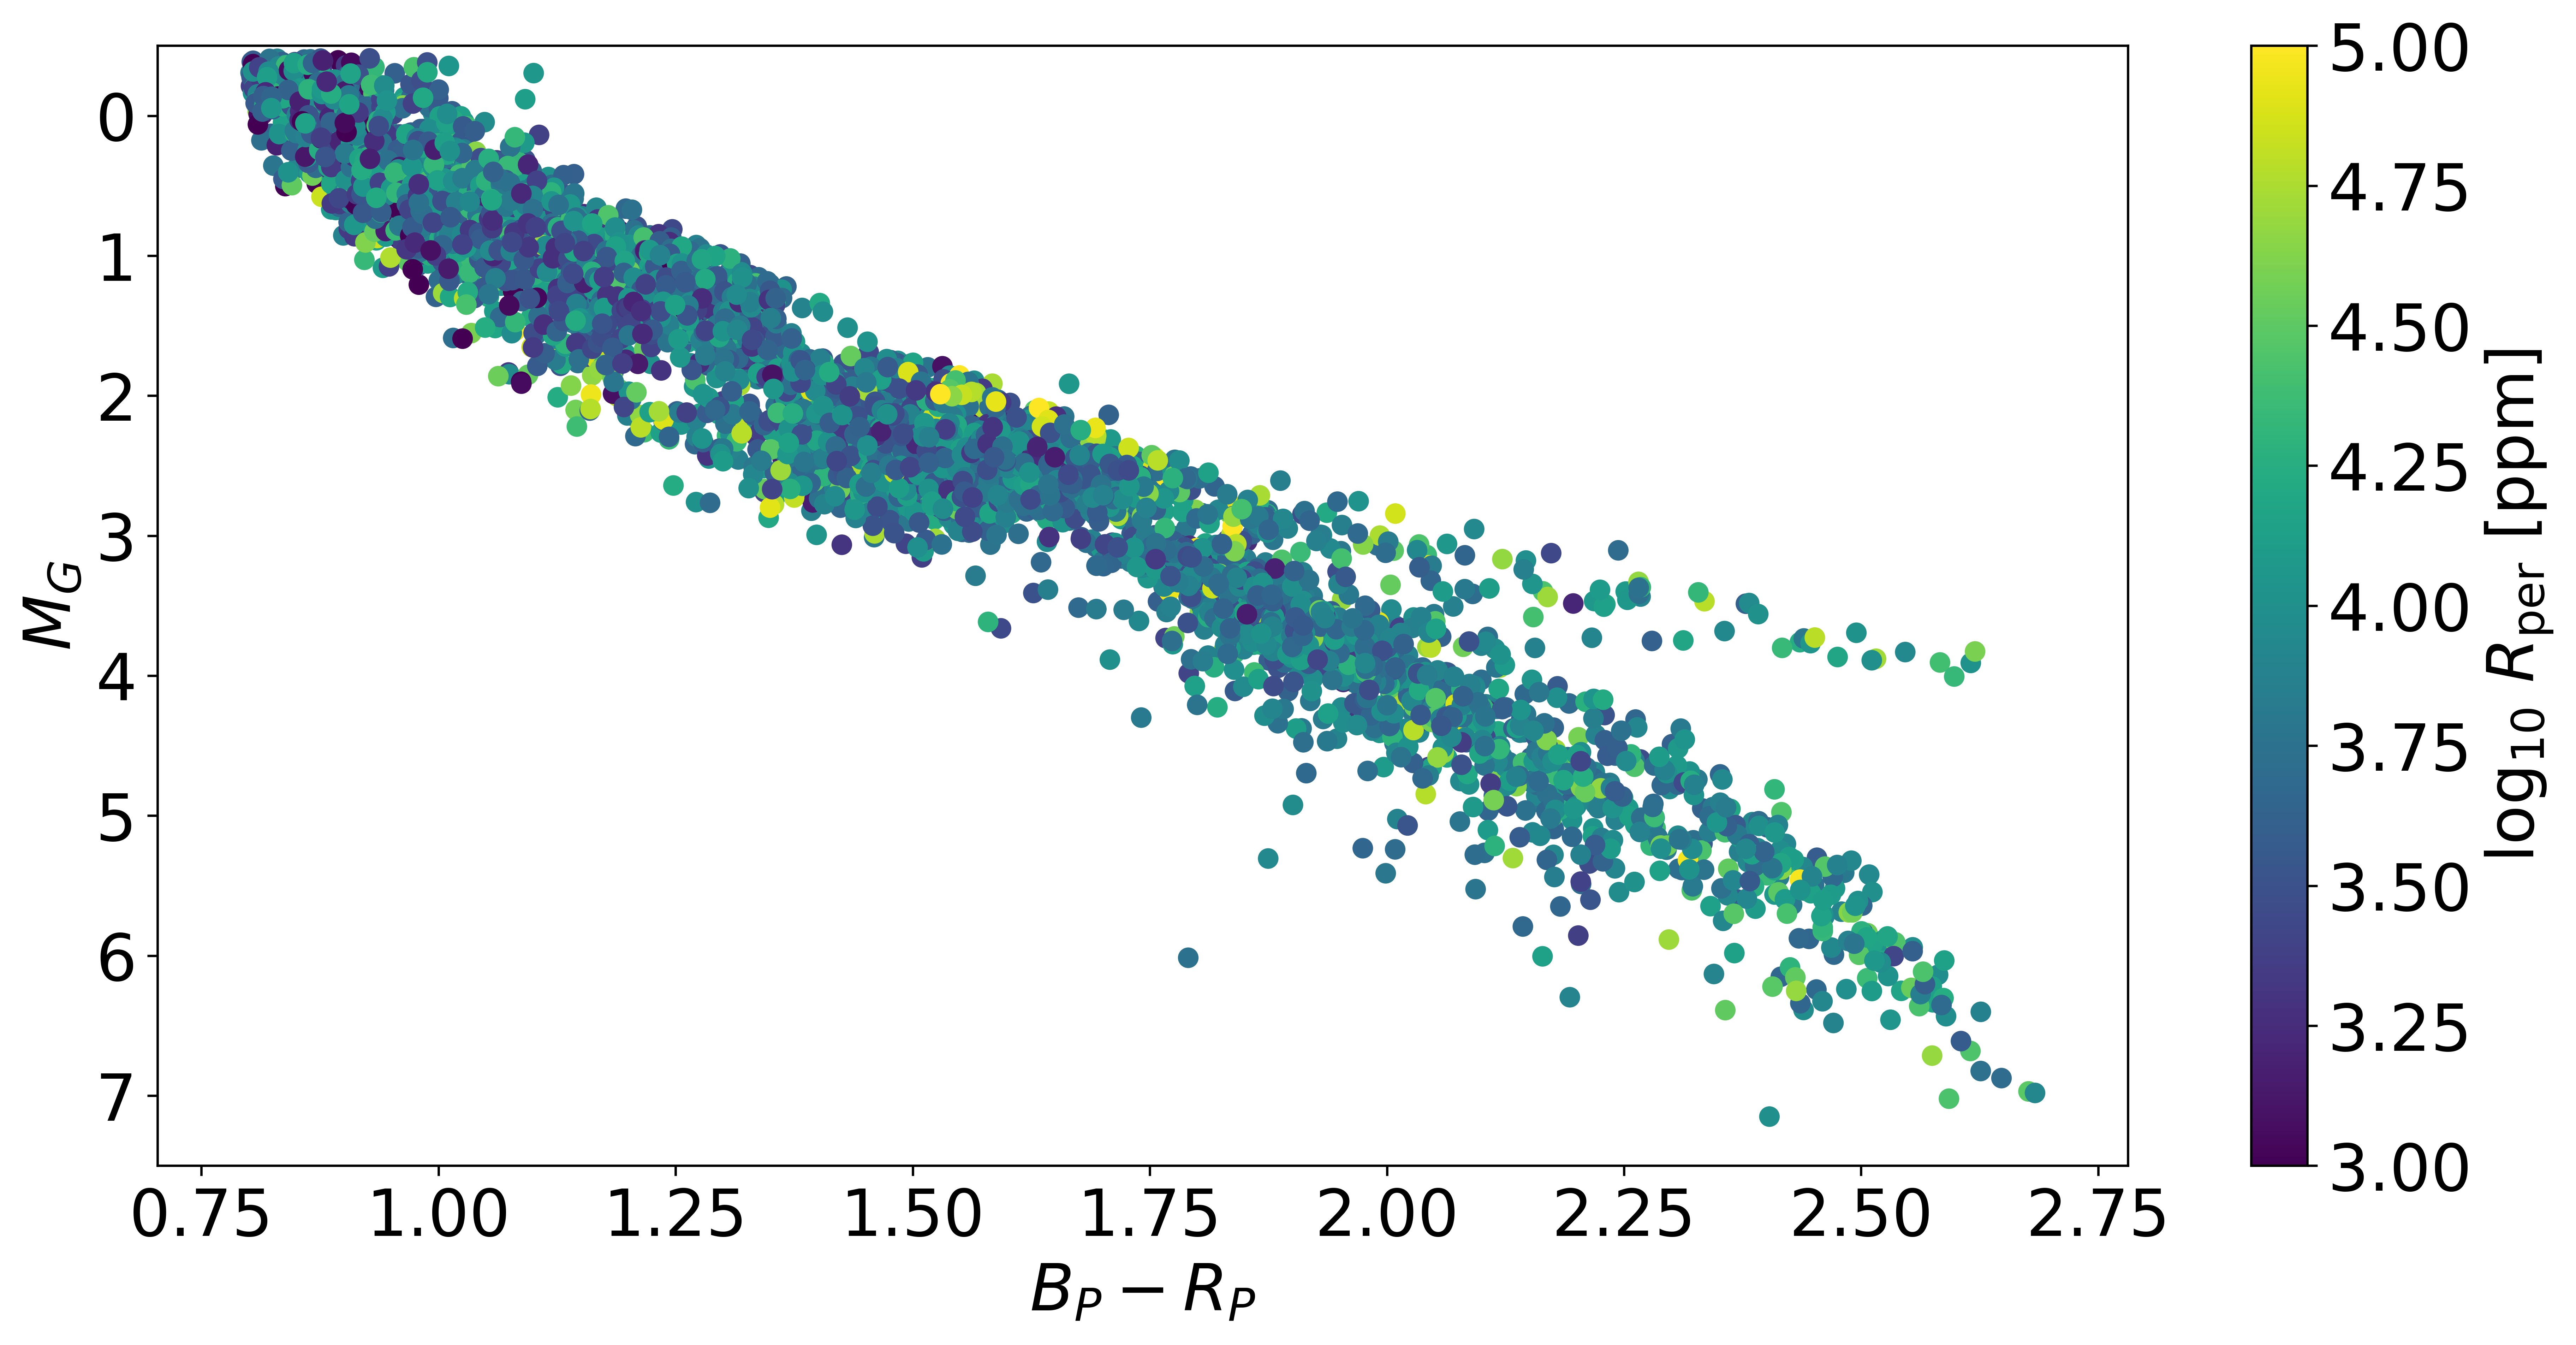
\includegraphics[width=\textwidth]{Figures/rot_gap_figures/HR.png}
  \caption{
  HR diagram of the closeby rotating main-sequence sample colours by photometric variability (\rper{}).}
  \label{fig:hr}
\end{figure}

\begin{figure}
\centering
  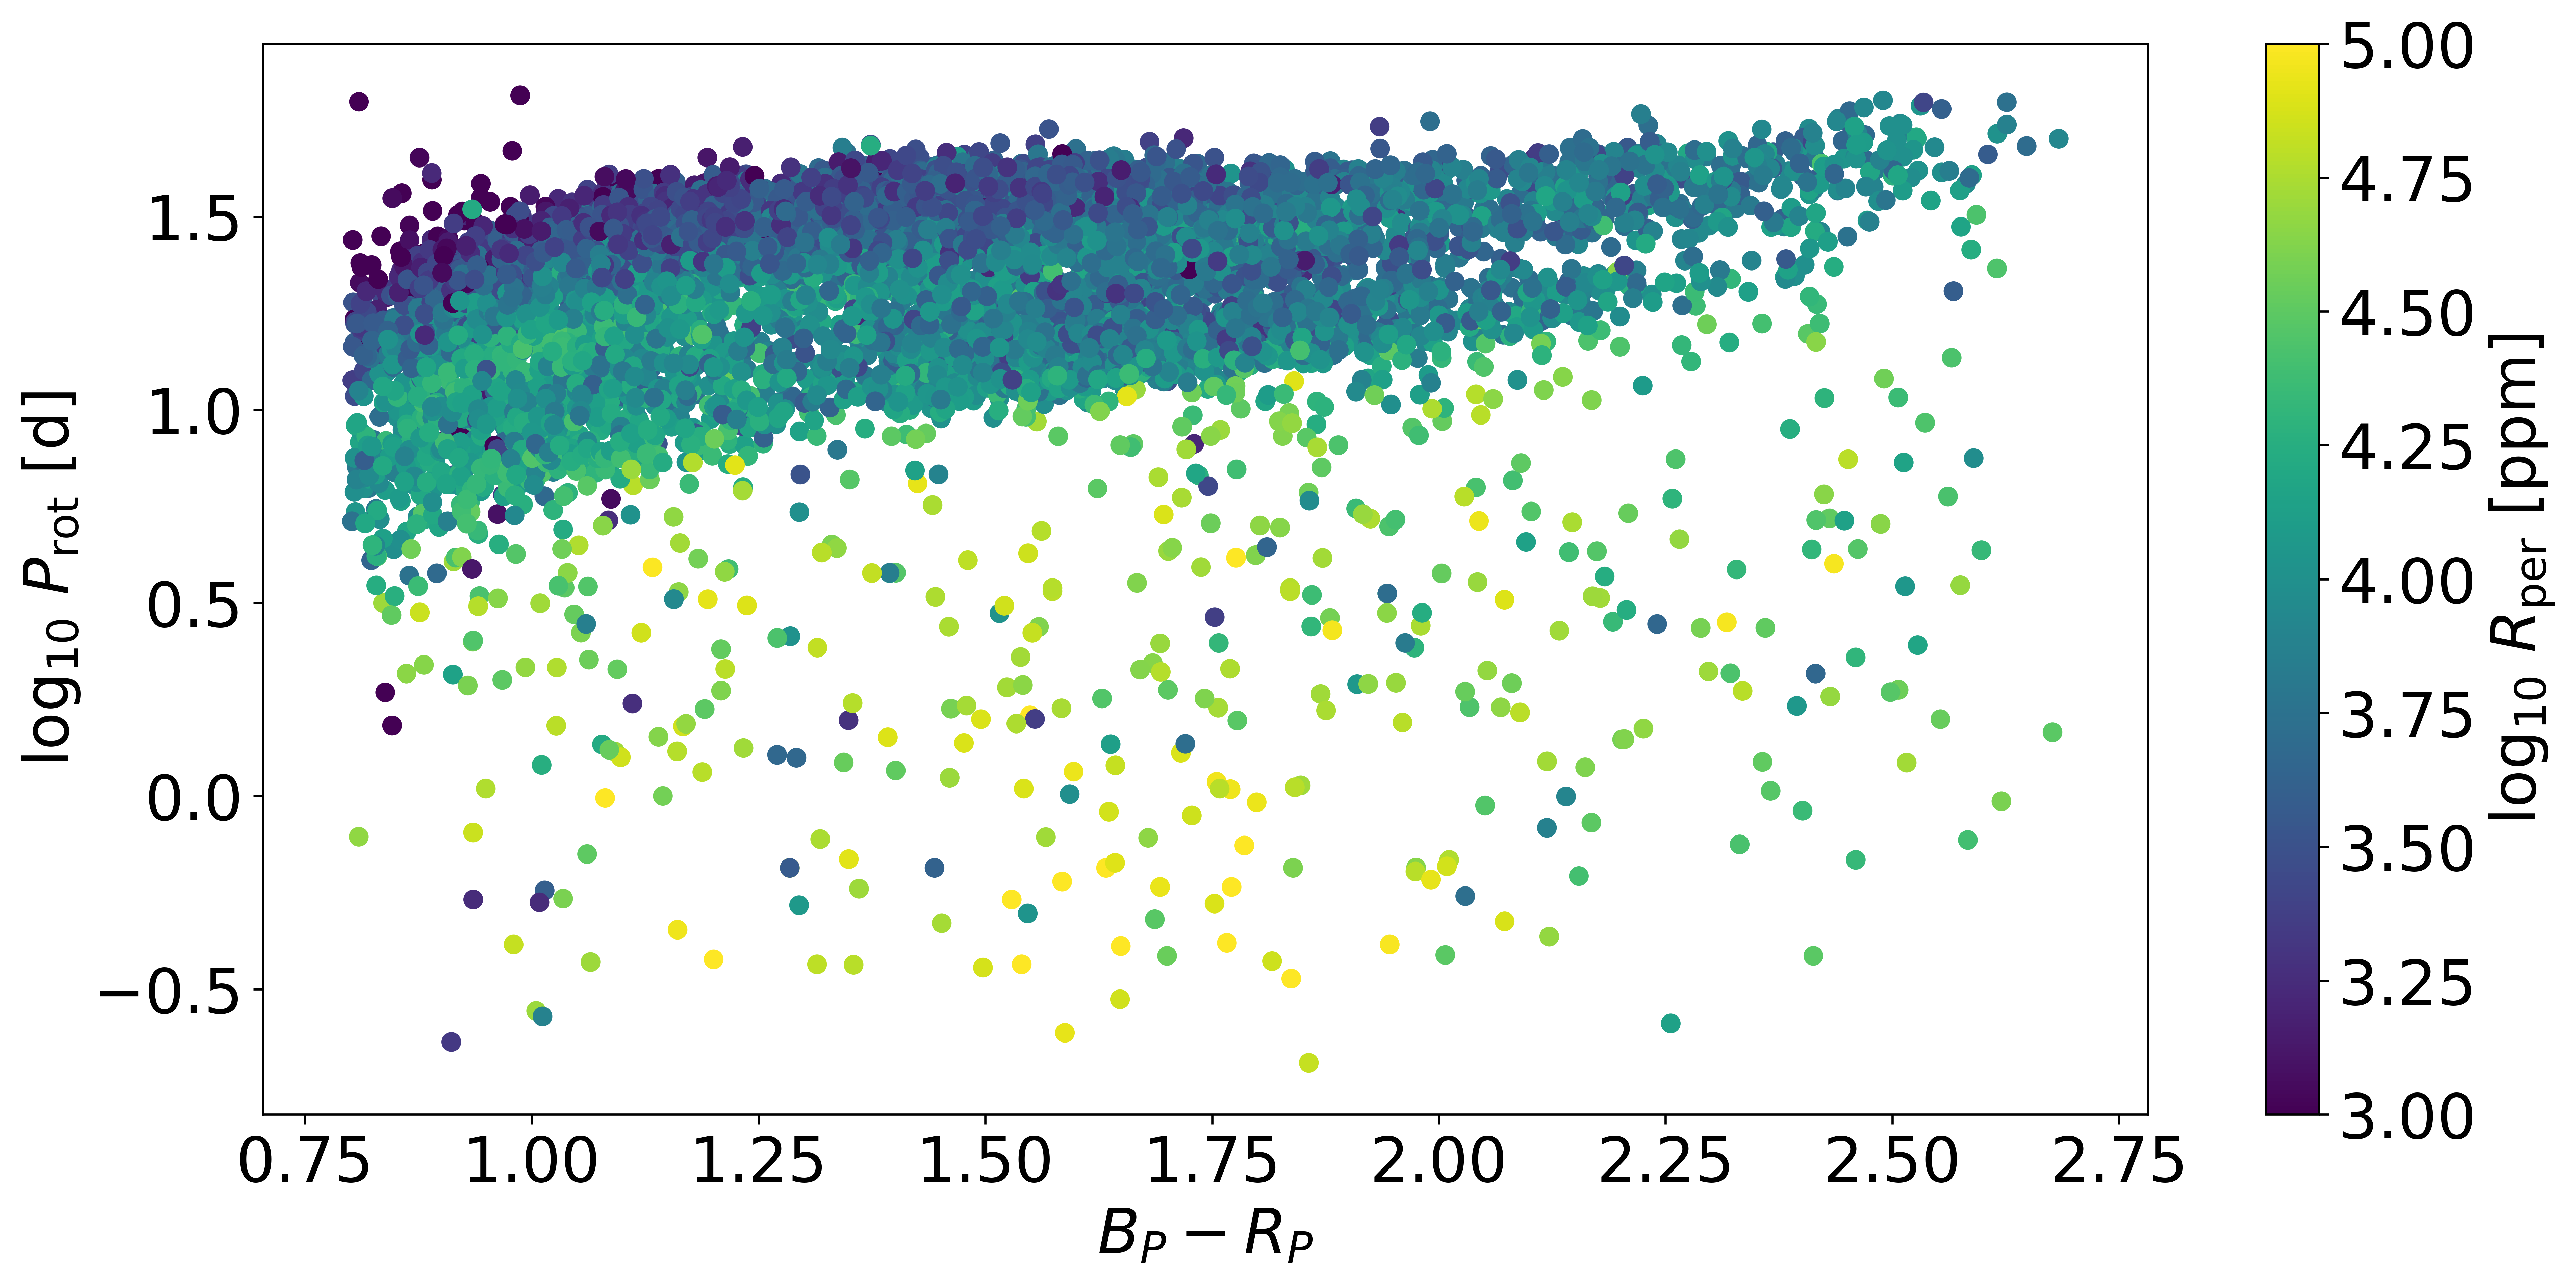
\includegraphics[width=\textwidth]{Figures/rot_gap_figures/rotational_dist.png}
  \caption{
  $\log_{10}$ of the rotation period against \gaia $B_P-R_P$ colour of the closeby rotating main-sequence sample colours by photometric variability (\rper{}). 
In this Figure, we can see observe the decrease in the photometric variability of stars near the gap.}
  \label{fig:prawn}
\end{figure}

From this sample, we can describe the average evolution of photometric variability around the intermediate period gap.
We will first separate the subsample into bins of $B_P - R_P$ (colour) from 0.8-2.5 of size 0.17 (10 bins).
In each colour interval, we then split the data into $log$ rotational period intervals of width 0.07 dex between 0.4 and 1.8 dex, corresponding to 2.5 and 70 days, respectively.
We then compute the median and median absolute deviation of \rper{} in each colour and rotational period bin.
The median is used here to attempt to alleviate the effect of activity cycles on the variance of the magnetic activity, and the median absolute deviation establishes the scatter on the measured photometric variability - regions with large median absolute deviation should be treated as less reliable measurements.
We neglected the regions with few stars ($<$5).
This removes the spurious stars that have not ascended onto the lower prong of the intermediate period gap, which does not indicate large-scale trends in the data.
We reconfirm that \rper{} tends to increase with mass, decrease with the rotational period, and decrease towards the rotational period gap \citep{reinhold_stellar_2020, basri_double_2018, santos_surface_2021}.
Comparing Figures \ref{fig:prawn} and \ref{fig:binned_rper_full_sample}, we also confirm that the gap aligns itself with a minima in \rper{}.

\begin{figure}
\centering
  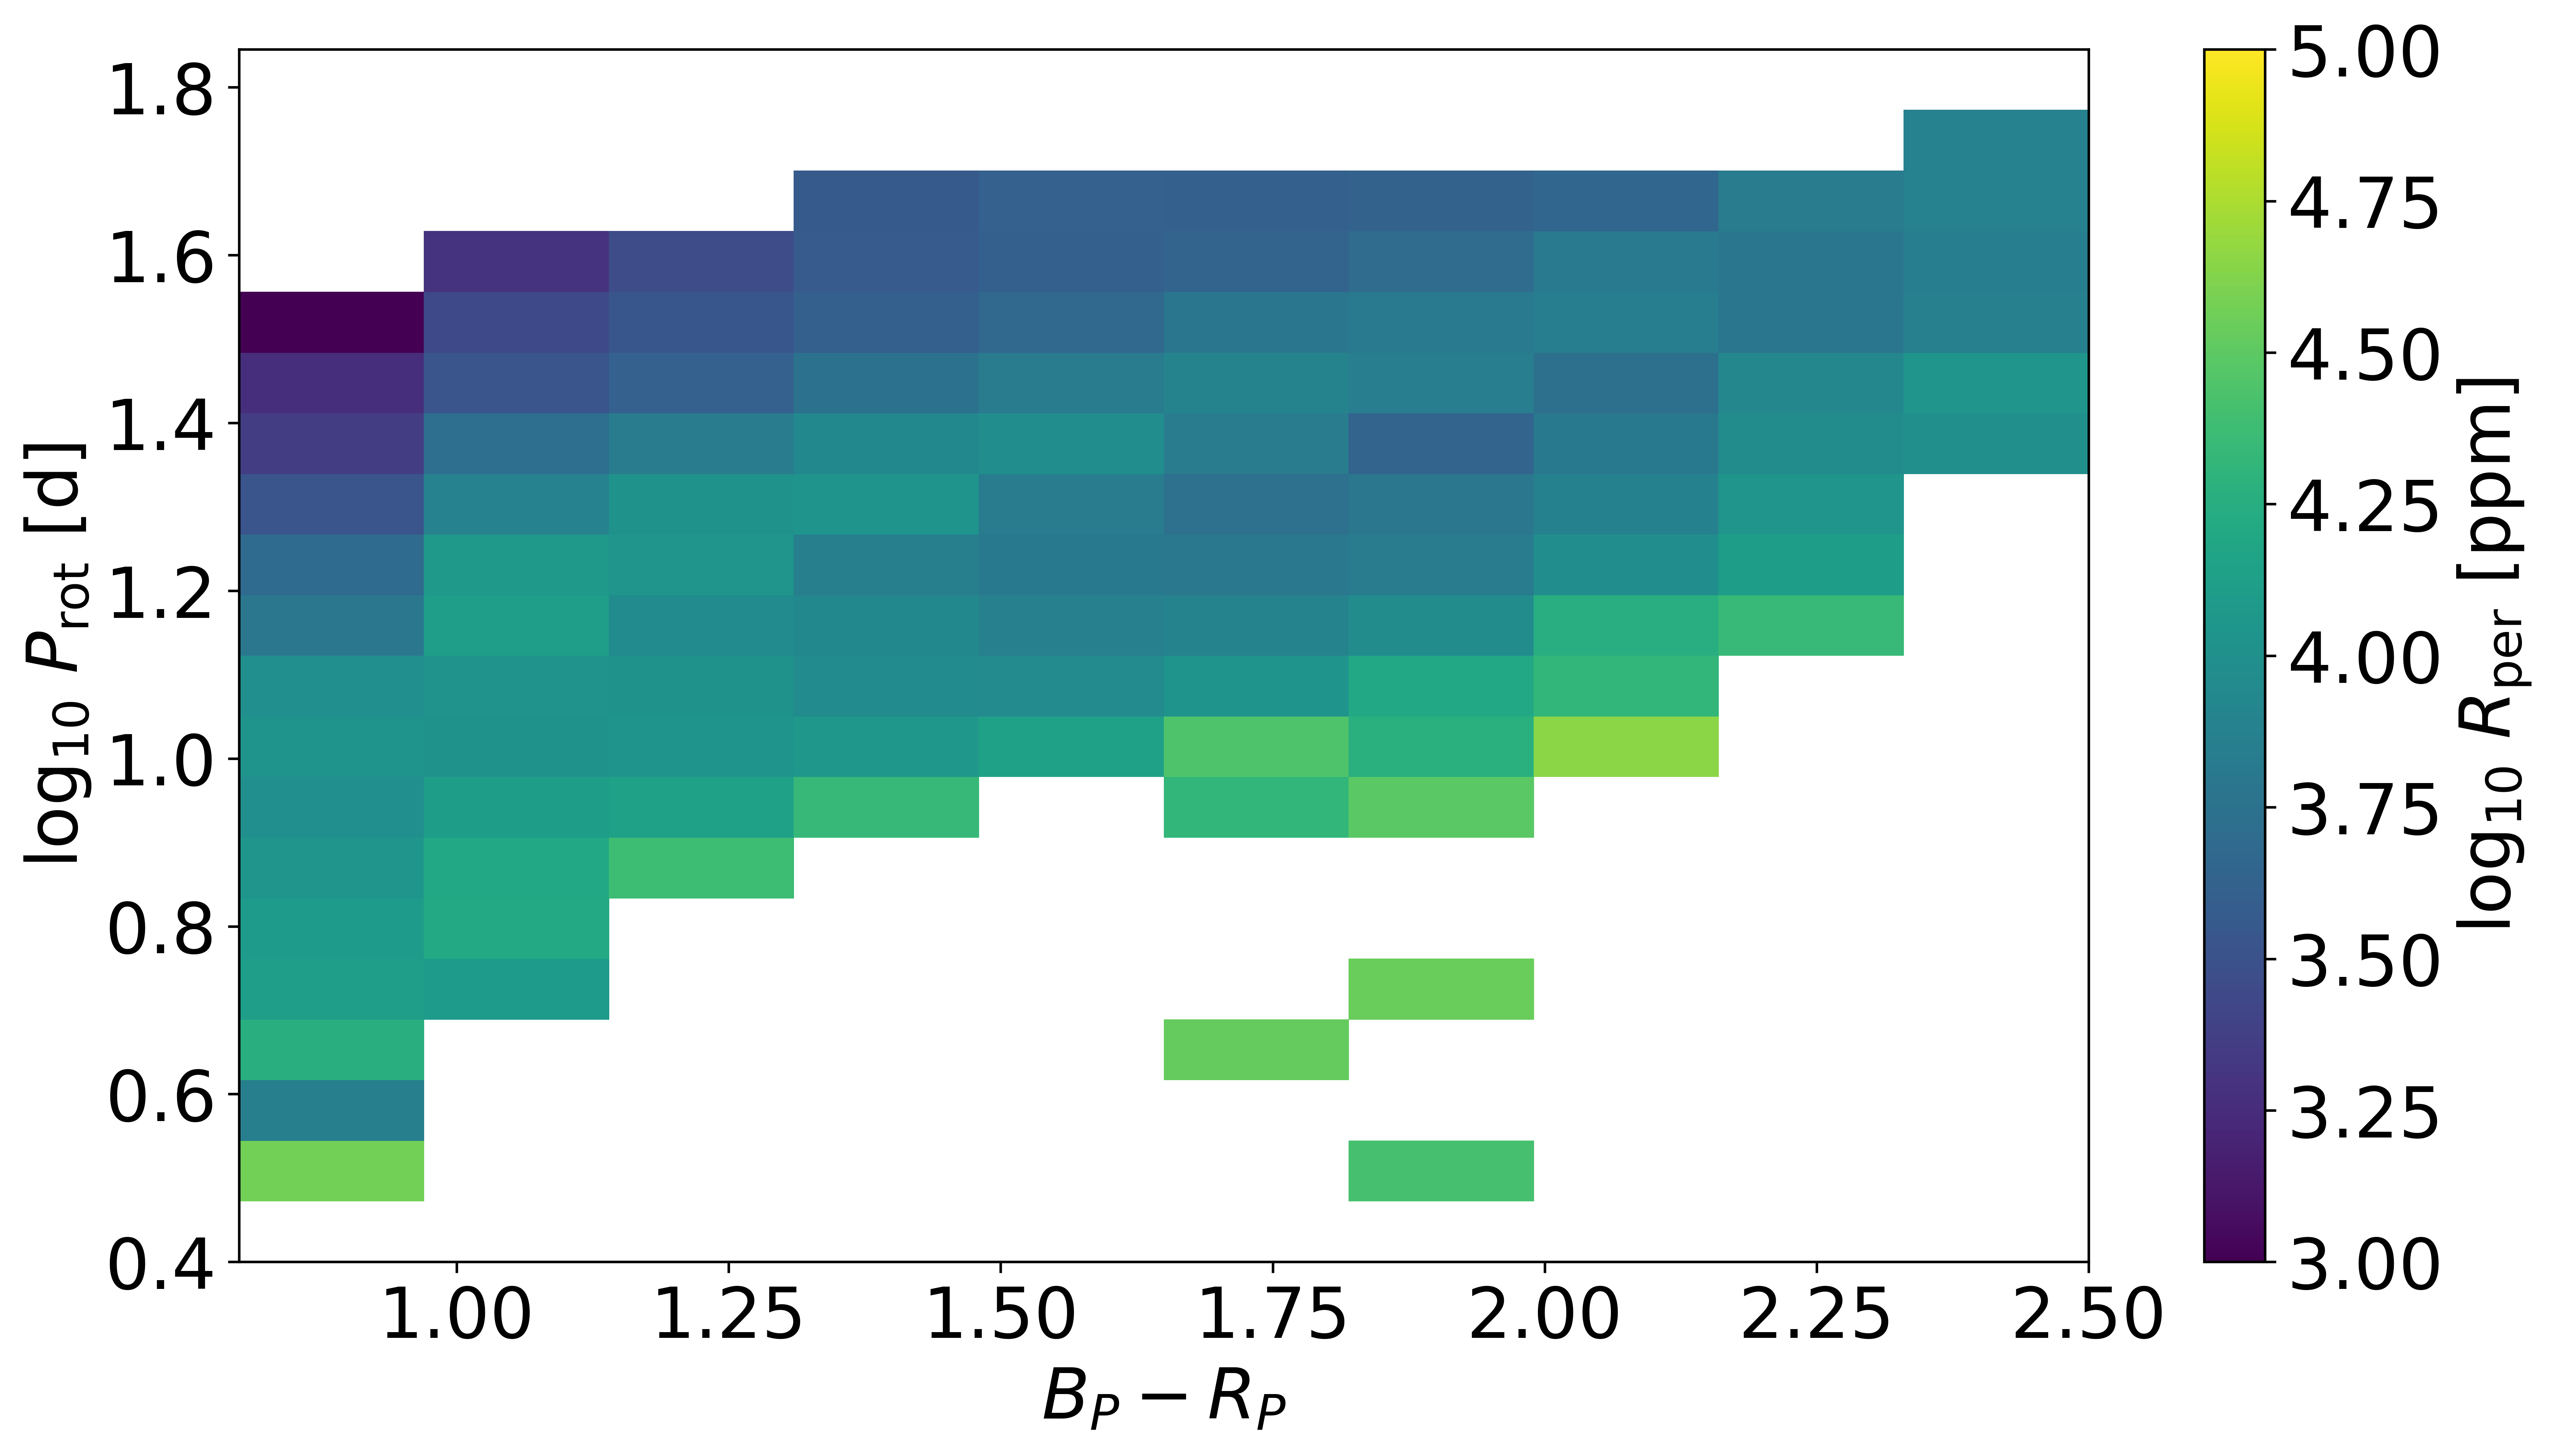
\includegraphics[width=\textwidth]{Figures/rot_gap_figures/rot_dist_binned.png}
  \caption{
  2D binned photometric variability (\rper{}) for the slices of $\log_{10}$ of the rotation period and colour \gaia $B_P-R_P$ used in this work. Comparing this Figure and \ref{fig:prawn}, the alignment of the minima of photometric variability and observation of stars in the gap can be seen.}
  \label{fig:binned_rper_full_sample}
\end{figure}

As a result of the large-scale variability with stellar mass and rotational period, the position of the minima becomes harder to notice as $B_P - R_P$ approaches 0.8.
We plot the same data in Figure \ref{fig:binned_rper_scatter} to make the minima more prominent.
We show the median \rper{} (scatter points) and scatter (errorbars) against the $\log_{10}$ of the rotation period for each colour range indicated in brackets - here, the colour of the interval increases down the plot - as well as fitted cubic spline to the data (dashed).
From the cubic spline, we can use the first and second derivatives of the spline to accurately determine the position of the local minima in \rper{}, which is indicated by the solid vertical blue line.

The calculation of the position of the minima is an automated process.
To identify minima, we calculate the first and second derivatives of the cubic spline fit and find where the first derivative is close to zero and where the second derivative is greater than 5 to ensure we ignore any spurious jitter in the spline fit.
We use an automated process to ensure we have not selected a position that we believe aligns with the intermediate period gap.
We found that the resulting position of minima can vary slightly depending on the smoothing of the cubic spline and the threshold value chosen for the second derivative.
However, the found minima here tended to be robust to variations of the smoothing at that threshold.
The first minima, in regards to the rotational period, in the $B_P-R_P =$ (0.8-0.97) bin was also manually ignored.

The position of the minima are shown in blue in Figure \ref{fig:indicating_minima}, where it is clear that the majority of minima align with the intermediate period gap.
We note that the minima do not accurately predict the position of the intermediate period gap for $B_P-R_P \geq 2.16$.
We believe this is because of the small number of stars below the gap in this colour range which were cut due to them not containing enough stars.
 With larger numbers of observations of low-mass stars below the gap we believe our prediction of the position of the rotation period gap with \rper{} \ would be more accurate in this regime. 
We also note that the average photometric modulation amplitude tends to peak to a maximum with a larger \rper{} than stars on the lower prong of the rotational period gap despite having longer rotation periods.
Whether this peak is indicative of stronger photometric activity suddenly above the gap or of suppression of photometric activity below the gap is unknown.

\begin{figure}
\centering
  \includegraphics[width=0.5\textwidth]{Figures/rot_gap_figures/rot_vs_rper_minima.png}
  \caption{
  Median and median absolute deviation of photometric variability (\rper{}) against $\log_{10}$ of the rotation period in bins of and colour \gaia{} $B_P-R_P$ (indicated in brackets). Here we have fitted a cubic spline to median \rper{} \ and calculated minima using the first and second derivatives of the fitted cubic spline. Solid vertical blue lines show the minima here. These minima align with the rotational period gap.}
  \label{fig:binned_rper_scatter}
\end{figure}

\begin{figure}
\centering
  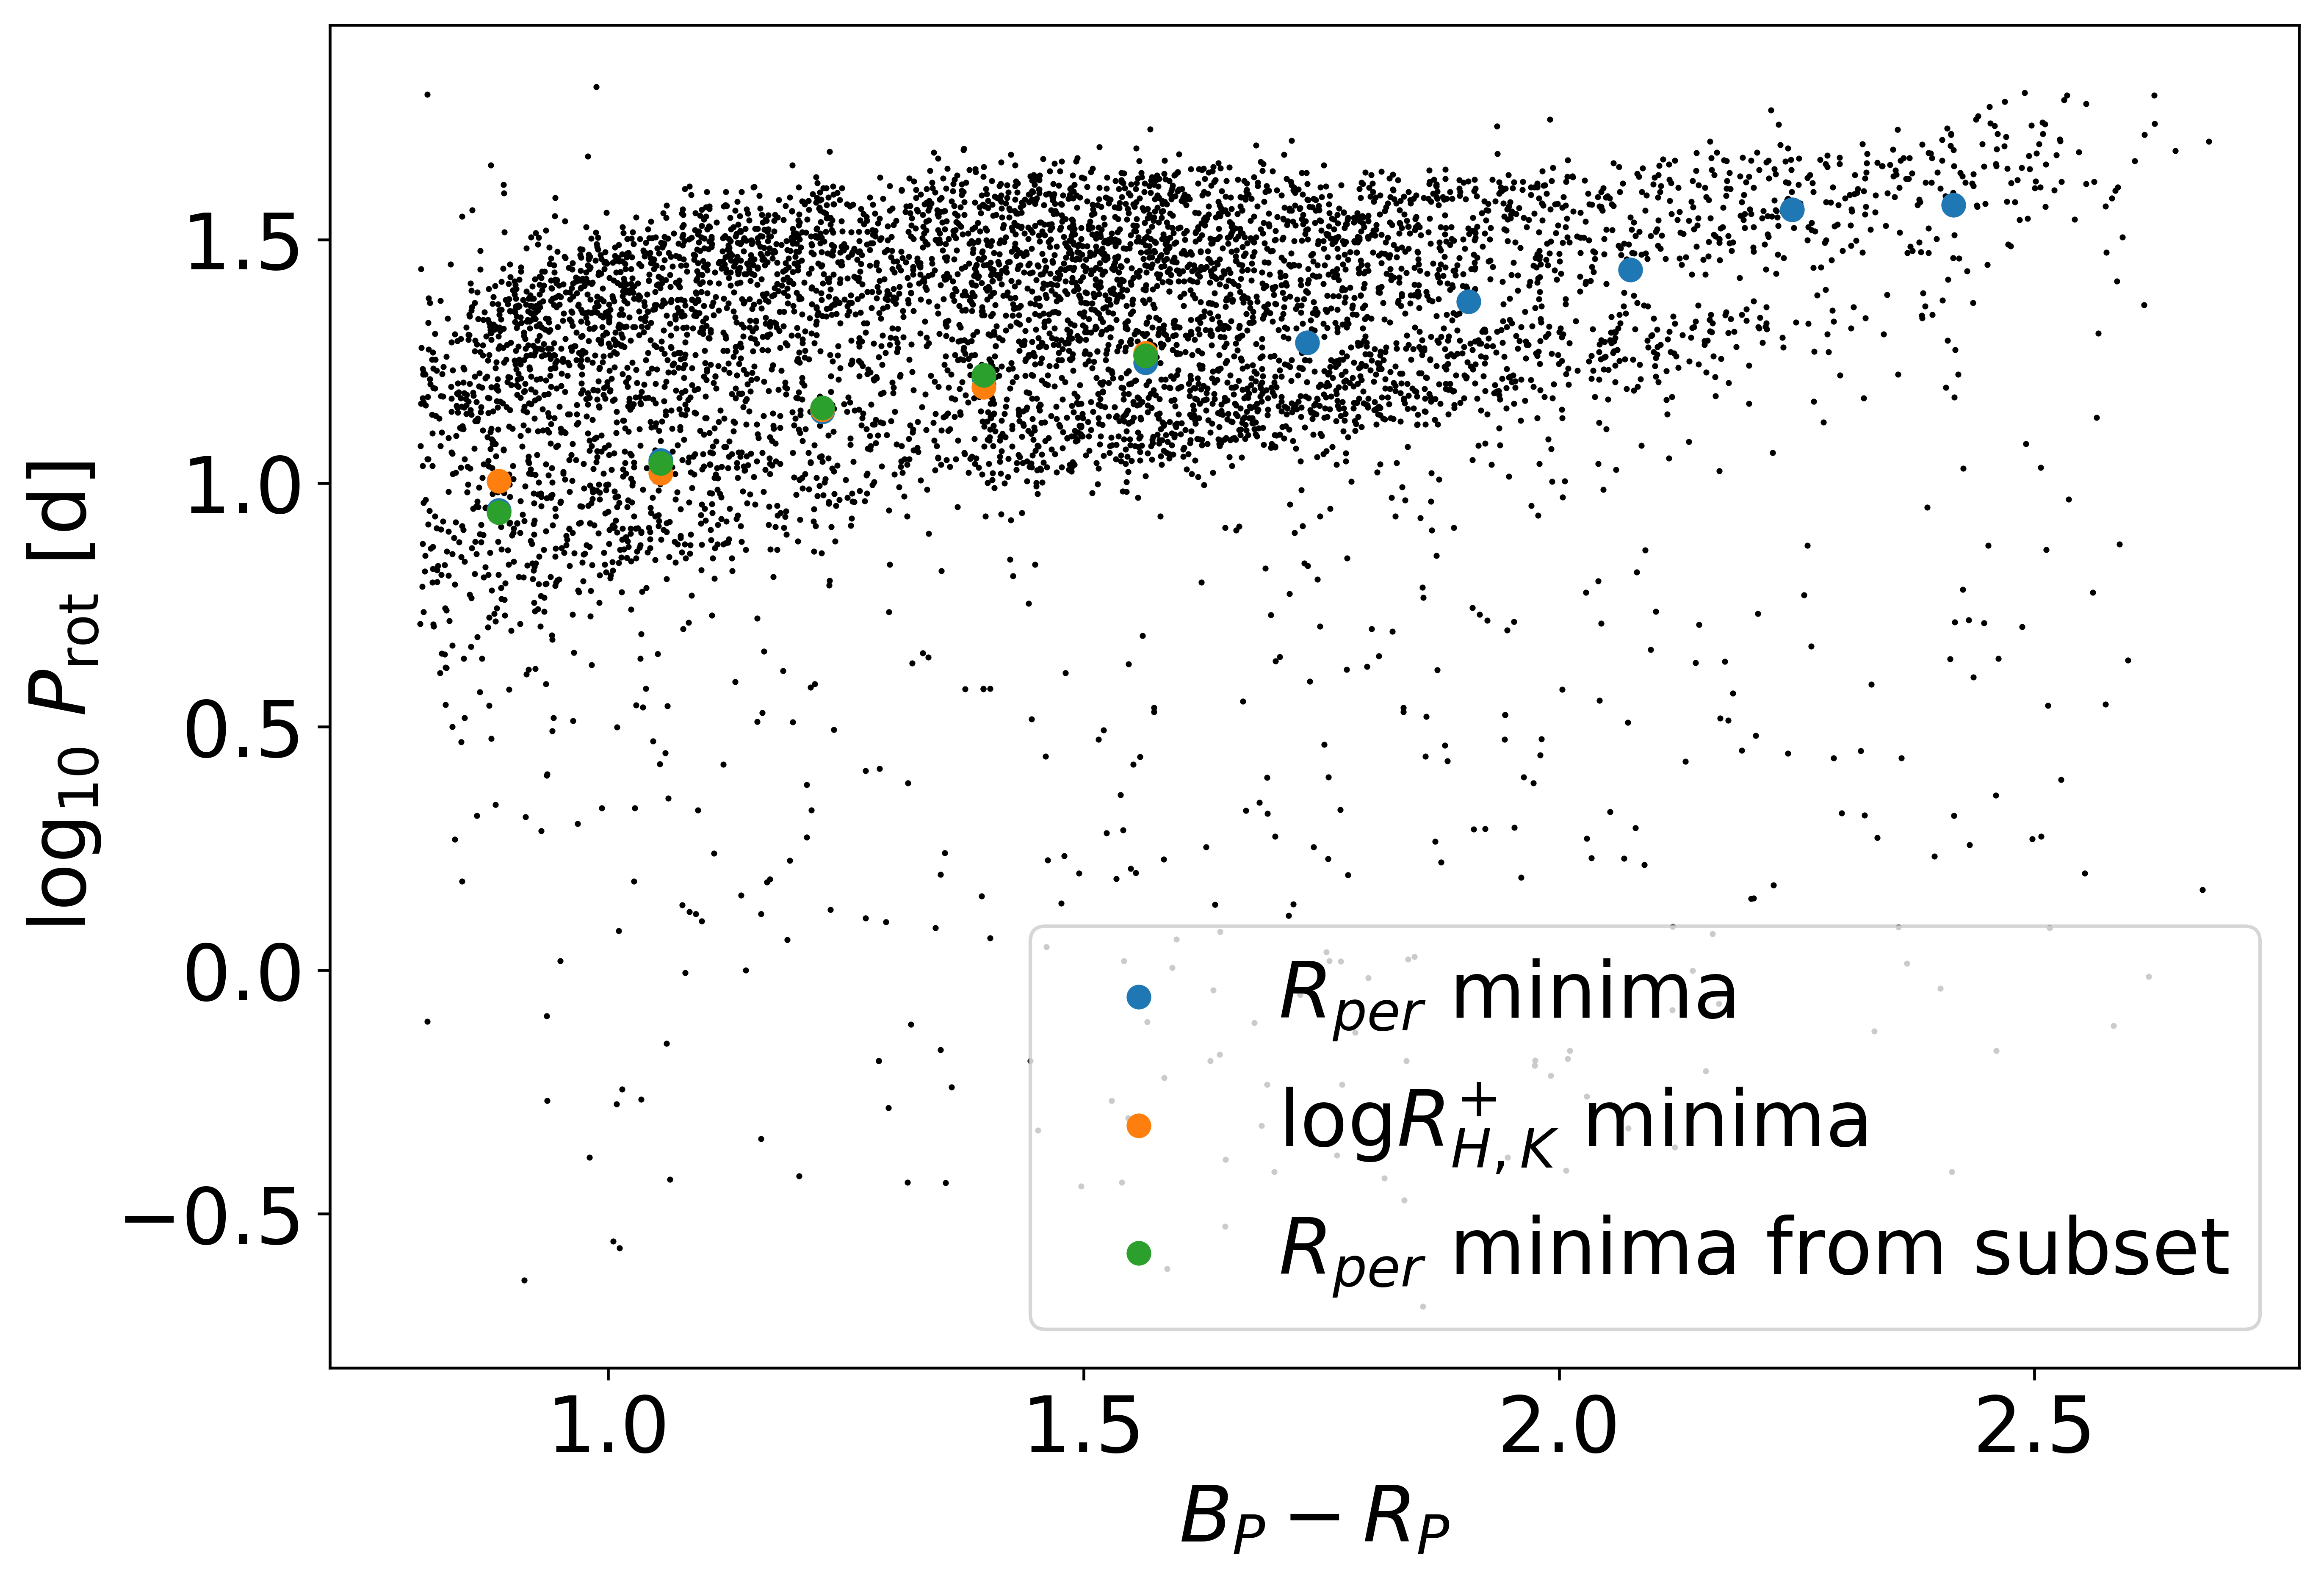
\includegraphics[width=\textwidth]{Figures/rot_gap_figures/rot_dist_minima_shown.png}
  \caption{
  The position of the identified minima in \rper{} \ against rotational period using the full close-by rotating main-sequence \kepler{} \ sample, the \rper{} minima identified with the \kepler{} LAMOST crossmatch and the $\log_{10} R^{+}_{H,K}$ minima identified with the \kepler{} LAMOST crossmatch.}
  \label{fig:indicating_minima}
\end{figure}

A possible explanation for the decrease in median photometric variability comes from the nature of a dearth of observations, as the gap is not horizontally aligned and increases in period for stars of lower mass (higher $B_P-R_P$).
\rper{} generally decreases with mass and rotation period.
Taking the median value in slices of constant rotation period near the dearth of observations will be systematically biased in different ways as it passes through the dearth.
In order of increasing rotation period, a sample of stars in each bin of rotation period will contain (1) majority fast rotating but redder stars and a small number of slow-rotating bluer stars, (2) approximately equal fast-rotating red stars and slow-rotating blue stars, and finally (3) majority slow-rotating bluer stars and a small number of fast-rotating redder stars.
The relationship between the \rper{} and mass or rotation period are not easily parameterised - especially near the gap.
However, we can confirm that this effect does not skew our results by calculating the median and median absolute deviation of $B_P-R_P$ in each colour and rotational period bin.
We have shown this in Figure \ref{fig:colour_rper}.
We confirm that the minima and maxima of \rper{} with rotation period in each colour bin do not correspond to minima or maxima in colour that would indicate that this effect is at play.
The variation is \rper{} is, therefore, a physical effect that aligns itself with the rotational period gap.

\begin{figure}
\centering
  \includegraphics[width=0.5\textwidth]{Figures/rot_gap_figures/per_vs_colour.png}
  \caption{
  Median and median absolute deviation of photometric variability (\rper{}) (blue) and $B_P-R_P$ (orange) against $\log_{10}$ of the rotation period in bins of and \gaia{} $B_P-R_P$ colour (indicated in brackets). The position of the minima in \rper{} \ do not align with maxima or minima in $B_P-R_P$ implying that the colour bias when fitting across the dearth can be the cause of the \rper{} \ minima.}
  \label{fig:colour_rper}
\end{figure}

At first glance, the minima in \rper{} surrounding the gap suggests that the rotation period gap is the result of the decreased probability of observing stars at the given rotation period.
However, the minima values of \rper{} within the gap can otherwise be detected for other colour stars.
For example, the minima in the $B_P-R_P$ - (0.97-1.14) slice has a \rper{} value of $\sim 4.0$, which can otherwise be easily detected for slower rotating or redder stars.
This either suggests that the periodic variability drops suddenly to levels where rotation is not measurable at the rotation period gap or that the rotational variability drops due to the process by which stars cross the gap. 
 \citet{santos_surface_2021} increased the sensitivity of period detection for \kepler{} lightcurves and did not increase the number of stars observed near the intermediate period gap - suggesting that the drop in photometric variability does not result in a decreased probability of observing stars near the gap.
This implies that if the drop in photometric variability is not the cause for the dearth of observations near the rotational period gap and rather that the drop in photometric variability is purely coincident with the rotational period gap - suggesting that the mechanism underlying the two observations is the same.
\rper{} is not defined for stars where rotation is not detected - as \rper{} is defined by the photometric variability range over a rotational period timescale.
Therefore we do not know whether the potential stars that lay within the gap, which we cannot observe because of the supposed dramatic decrease in \rper{}, do or do not suddenly decrease in \rper{}.

\section{The gap aligns with a minima in $\log R^{+}_{\rm{HK}}$ }
\label{sec:minima_rhk}

While it has been well established that the photometric variability of stars decreases towards the intermediate period gap other magnetic activity indicators have not been explored in this regard, only the large-scale trends with stellar mass and rotation \citep{zhang_magnetic_2020}.
Suppose other magnetic activity indicators vary in the same fashion as \rper{} - decreasing to a minimum at the rotational period gap. 
In that case, it is more likely that the decrease in \rper{} towards the gap results from a variation in the magnetic field of stars.
We will begin by testing whether this is indeed the case.

\citet{zhang_magnetic_2020} extracted the chromospheric magnetic activity indexes, S and $\log \ R^{+}_{HK}$, for 59,816 stars from low-resolution LAMOST spectra in the LAMOST-Kepler program.
The crossmatch of their work with the nearby rotating main sequence we established yielded 1060 stars.
The stars in the crossmatch tend to be the higher mass, brighter stars with $B_P-R_P<1.8$, where the intermediate period gap is less apparent.
Given that we could predict the gap position for these stars in our earlier experiment, we carry forward and re-analyse their data under a new framework.

$\log \ R^{+}_{HK}$ provides a more accurate measure of the chromospheric magnetic activity than $S$, which is uncoupled from a radiative contribution, so we adopt $\log \ R^{+}_{HK}$ in this work.
The resulting rotational distribution of stars is shown in Figure \ref{fig:rot_dist_rhk} coloured by $\log \ R^{+}_{HK}$.
Due to the smaller number of stars and lower precision of $\log \ R^{+}_{HK}$ than \rper{} it is not clear whether $\log \ R^{+}_{HK}$, like \rper{} decreases towards to the intermediate period gap.


\begin{figure}
\centering
  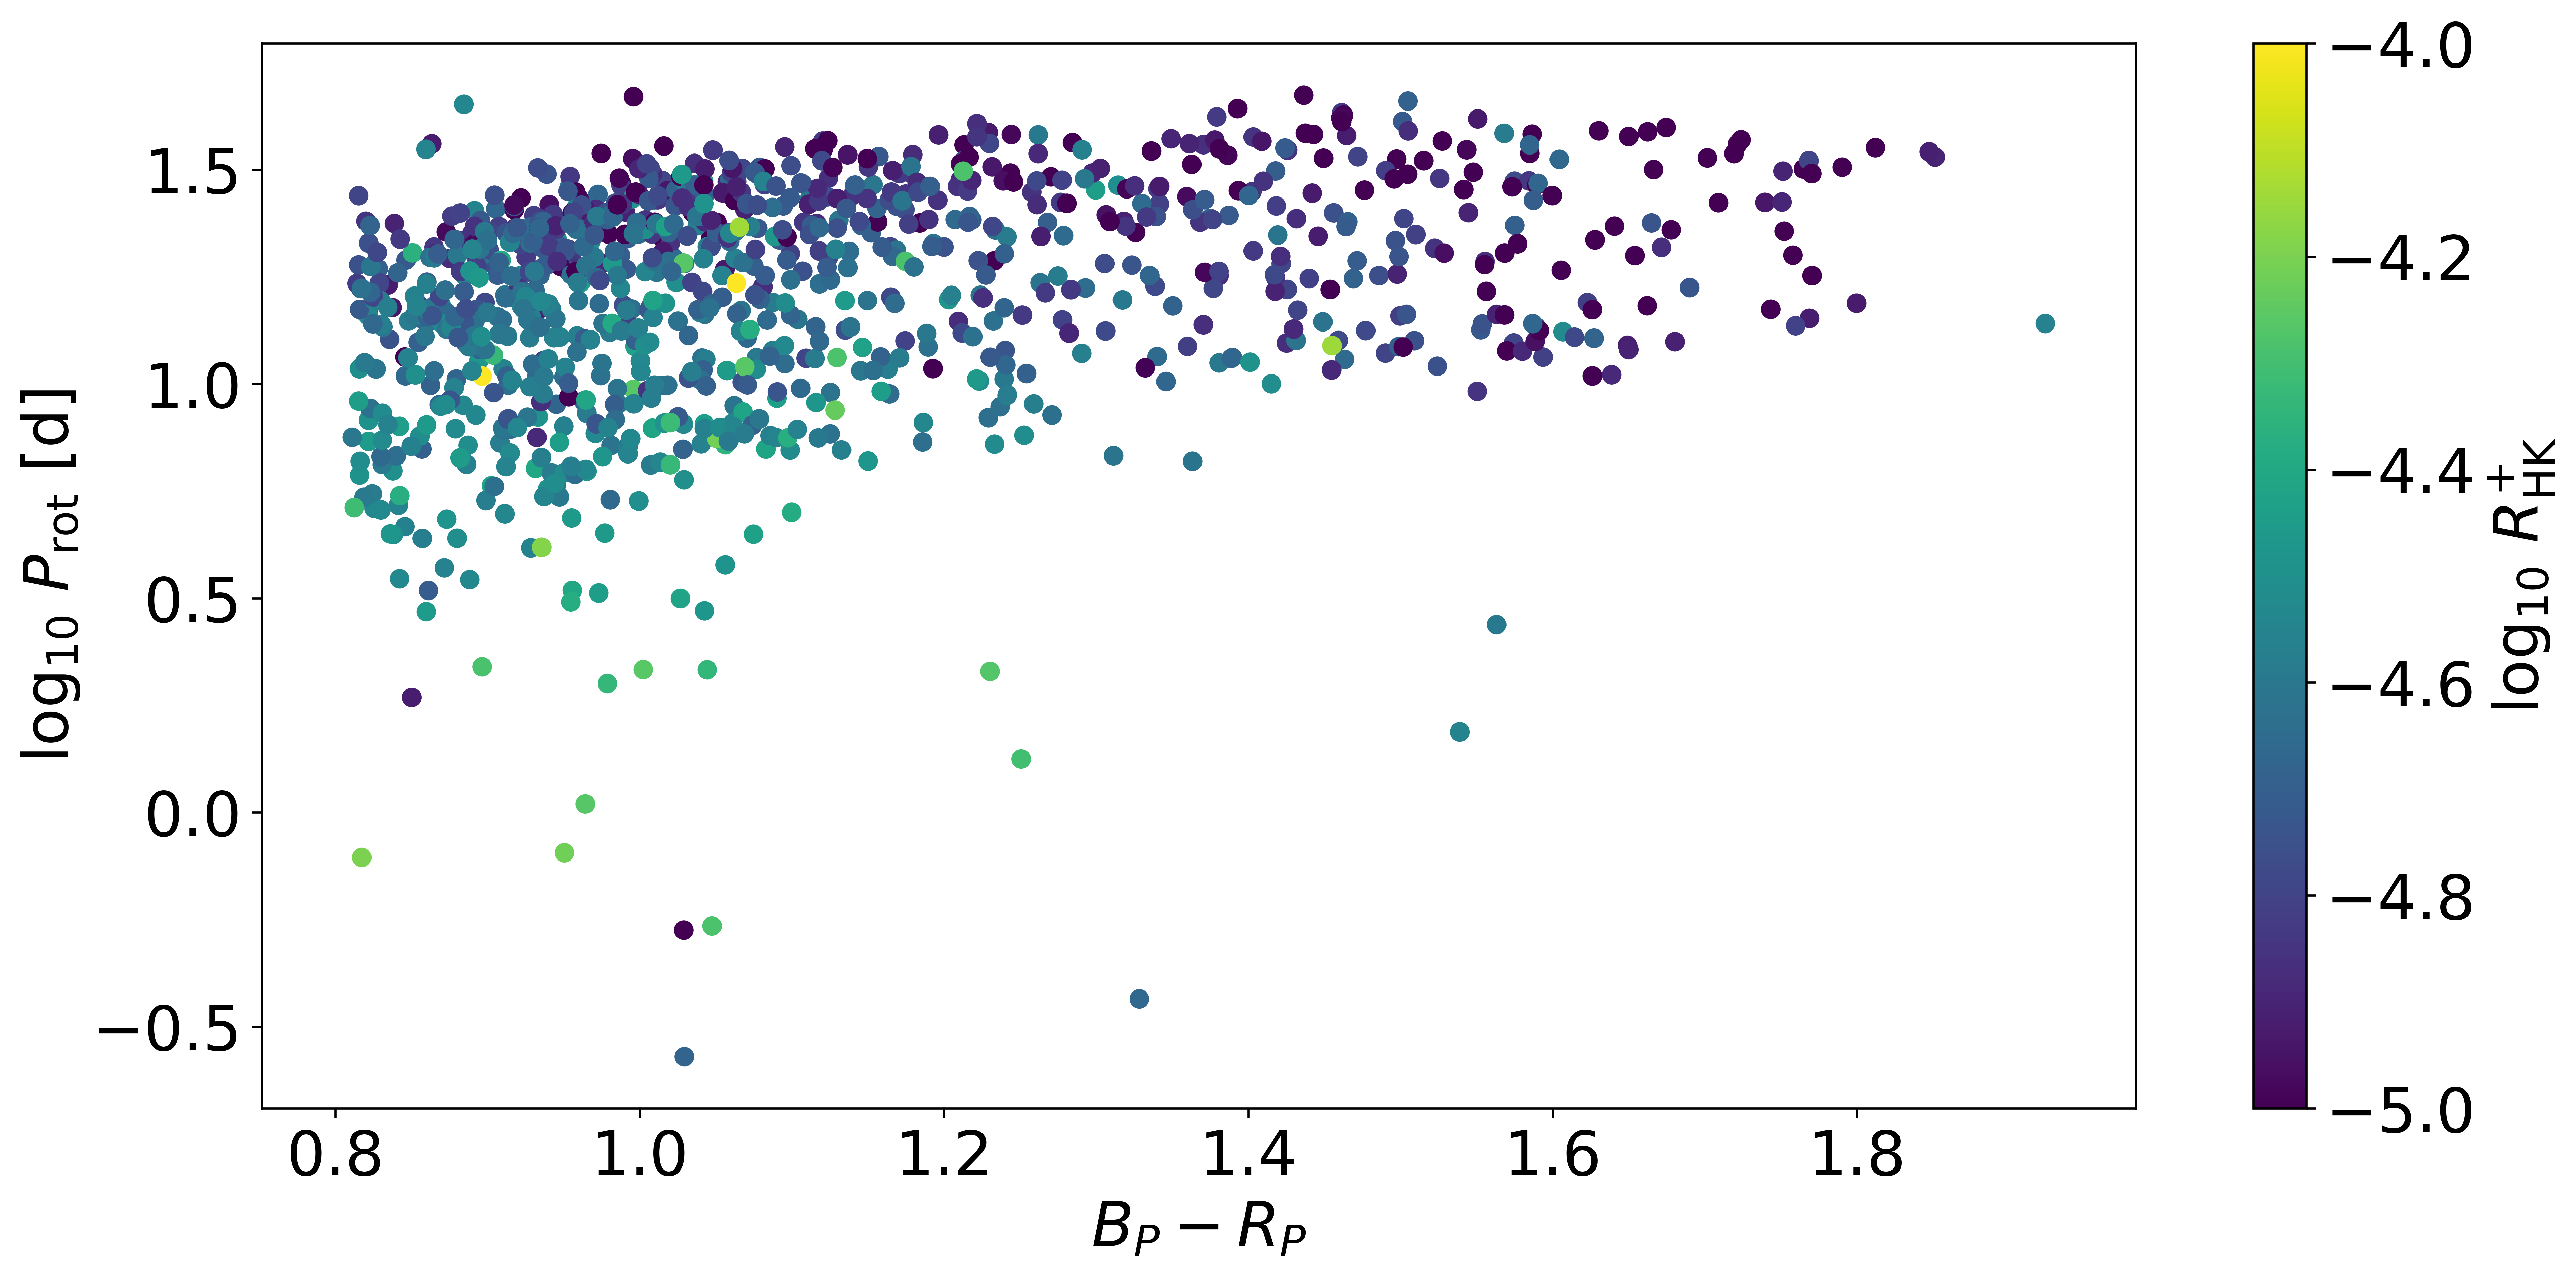
\includegraphics[width=\textwidth]{Figures/rot_gap_figures/rotational_dist_rhk.png}
  \caption{
  The LAMOST chromospherically active and \kepler{} rotating closeby, main-sequence cross-match $\log_{10}$ of rotational period $\log_{10}$ against \gaia $B_P-R_P$ colour coloured by $\log_{10}R^{+}_{\rm{HK}}$. It is unclear from this whether $\log_{10}R^{+}_{\rm{HK}}$ decreases toward the gap like \rper{}.}
  \label{fig:rot_dist_rhk}
\end{figure}

To determine this more concretely, we adopt the same process as we described earlier to find the minima in \rper{} \ in a bin of colour against the rotational period.
We again separate the stars into the same slices of $B_P-R_P$ and log of rotation period, and remove any bins containing small numbers of stars ($<$2).
This cut-off was chosen because of the reduced number of stars in the sample \kepler{}-LAMOST crossmatch, compared to the \citet{mcquillan_rotation_2014} sample.
 Still, the results should be treated with more caution because we rely on small number statistics.
The median and median absolute deviation of both $\log \ R^{+}_{HK}$ and \rper{} \ in these slices was then calculated, which we then fit with cubic splines against the log of the rotation period.
We have repeated this method on \rper{} \ here because we are using a subset of the original stars and to compare the recovered minima from the subset more accurately - this also allows us to confirm the accuracy of the fit of our minima in the first test.
The minima of the cubic spline fits are then calculated again using the first and second derivatives using the same smoothing and first and second derivative thresholds.

\begin{figure}
\centering
  \includegraphics[width=\textwidth]{Figures/rot_gap_figures/rot_vs_rper_rhk_minima.png}
  \caption{
  Median and median absolute deviation of photometric variability (\rper{}) (blue) and LAMOST $\log_{10}R^{+}_{\rm{HK}}$ against $\log_{10}$ of the rotation period in bins of and colour \gaia{} $B_P-R_P$ (indicated in brackets). Here we have fitted a cubic spline to the median of these values in each bin and calculated minima using the first and second derivatives of the fitted cubic spline. The minima in \rper{} are shown by solid vertical blue lines, while the minima in $\log_{10}R^{+}_{\rm{HK}}$ are shown in solid vertical orange lines. These minima align with each other and the rotational period gap.}
  \label{fig:rot_rper_rhk}
\end{figure}

We compare the distributions of \rper{} \ and $\log \ R^{+}_{HK}$ against the log of rotation period in Figure \ref{fig:rot_rper_rhk} and show the found minima in blue and orange solid vertical lines for \rper{} \ and $\log \ R^{+}_{HK}$ respectively.
Like photometric variability, $\log \ R^{+}_{HK}$ tends to decrease with rotational period - owing to their relation to the strength of the magnetic field.
We find that, generally, \rper{} \ and $\log \ R^{+}_{HK}$ are directly tied - increases and decreases to the median value with rotational period in one tends to align with a similar response in the other.

We show the comparison of the recovered minima from \rper{} using this subset as well as the minima recovered using $\log \ R^{+}_{HK}$ in Figure \ref{fig:indicating_minima}.
The recovered \rper{} \ minima using the subset lay on top of the \rper{} minima recovered using the full sample.
Interestingly, we may detect previously unreported minima in $\log \ R^{+}_{HK}$ close to the rotation period gap.
Excluding the minima recovered in the $B_P-R_P$ - (0.8-0.97) bins, the minima that we recover in $\log \ R^{+}_{HK}$ against logged rotational period are in the same period bin and are close in position to the minima of \rper{} we recover, which we have established aligns with the intermediate period gap.
The alignment of the minima is also robust to variation in the smoothness of the fitted cubic spline - suggesting that the minima are not spurious.

Measurements of $\log \ R^{+}_{HK}$ are less precise than \rper{}, which is reflected in the relatively larger median absolute deviation.
The detection of the coincidence in a single slice of $B_P-R_P$ could be explained through this imprecision.
Alternatively, the coincidence of the two may simply be a coincidence.
Detecting this in multiple slices of $B_P-R_P$ suggests that the cause of the minima is related.
Further study of this relationship is required to confirm the coincidence of the minima with a larger dataset of chromospheric magnetic activity indicators or with other magnetic activity indicators.
We will assume, for now, that the rotational period gap does align itself with minima in both \rper{} and $\log \ R^{+}_{HK}$ and explore whether there is a sample of low-magnetic activity, non-detected rotators.

\section{Is there a sample of low-magnetic activity stars without rotational period detection?}
\label{sec:low_activity_gap}

If the gap contains stars that have dramatically low \rper{} and thus do not have detectable rotation periods, then $\log \ R^{+}_{HK}$ should also dramatically drop within this regime.
If there is a sample of dramatically lower $\log \ R^{+}_{HK}$ stars without detected rotation periods, then the existence of such a subsample would support the hypothesis that the intermediate period gap results from a decreased probability of observing stars at those rotation periods due to a decrease in stellar activity.

%To determine whether a star has a significant rotational period detection \citet{mcquillan_rotation_2014} defines a weight of the significance of the detection of the rotational period $w$ and compares this to a threshold value.
%$w$ is defined in terms of the ACF's local peak height (LPH), the height of the selected peak with respect to the mean of the troughs on either side, the star's temperature and the rotational period.
%For a more thorough description of their method for calculating this value see Section A in the appendix of their work.
%This normalised value is calculated for each star and compared to a threshold value.
%Those that do not pass the threshold were placed into a separate category of stars that do not have a detectable rotation period.

We will compare the $\log \ R^{+}_{HK}$ distributions of the \citet{mcquillan_rotation_2014} rotating and non-rotating samples.
We prepare the sample of 99,000 stars without detected rotation periods from their work\footnote{This is a slight misnomer as \textit{some} of the stars $\sim$ 100,000 stars have detectable rotation periods, but do not pass a detectability threshold, see Section A in the appendix of their work, and those periods should be treated with some care.} in the same way that we did for the rotating sample - ensuring they are close by ($<525 pc$), on the main-sequence and redder than $B_P-R_P$ = 0.8 where the rotational period gap is most apparent.
This leaves us with a sample of 5574 non-rotating close by, main-sequence stars, which we can cross match with the LAMOST-\kepler{} \ sample of chromospheric active stars measured in \citet{zhang_magnetic_2020} - reducing the number of stars to 1134 stars.
The number of stars in this sample is similar to that in the rotating sample.
We show the resulting HR diagram of stars without rotational detection (bottom) and with rotational detection (top) in Figure \ref{fig:non_rotating_mag_hr} coloured by $\log \ R^{+}_{HK}$.
Comparing the distributions, it is clear that the non-rotating sample is clearly biased for higher mass stars and does not permeate into the low mass regime, where the gap would be most apparent.

\begin{figure}
\centering
  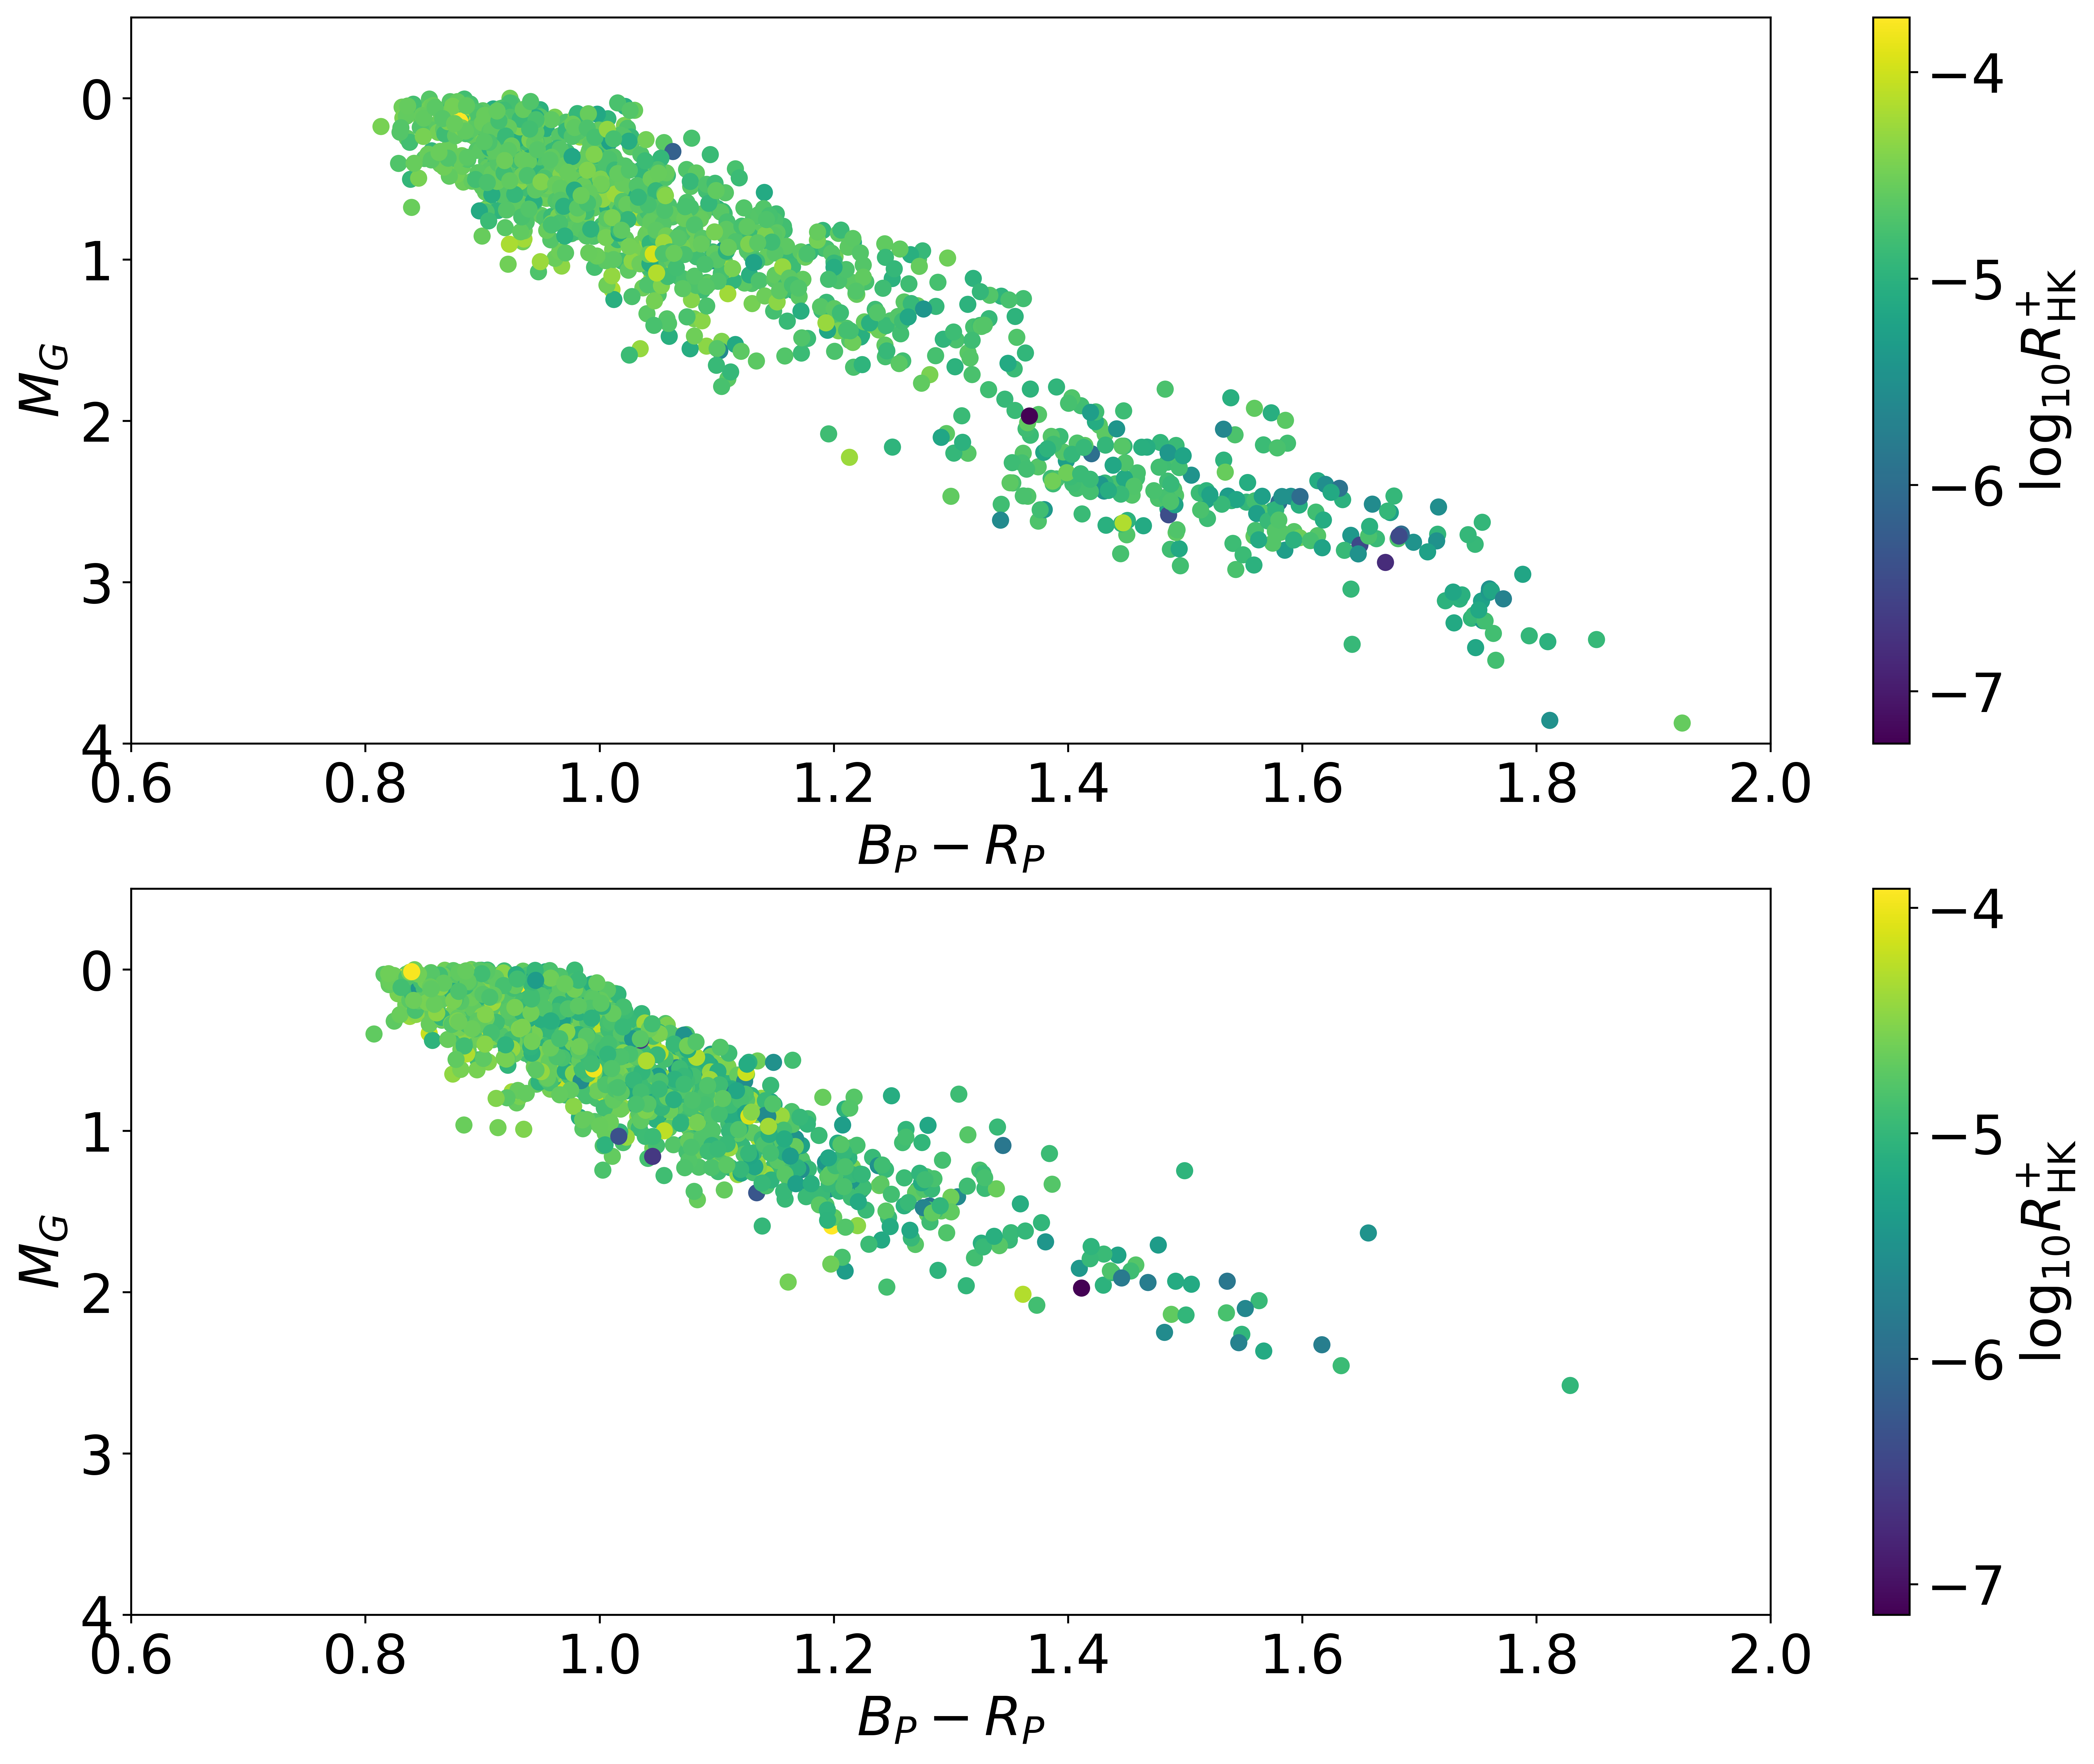
\includegraphics[width=\textwidth]{Figures/rot_gap_figures/HR_mag_and_non_rot.png}
  \caption{
  HR diagram of the closeby rotating (top) and non-rotating (bottom) main-sequence sample crossmatched with the LAMOST-\kepler{} field coloured by the chromospheric magnetic activity indicator $\log \ R^{+}_{HK}$.
  Comparing these two samples, we observe very few low-mass stars for which the rotation period is undetected.}
  \label{fig:non_rotating_mag_hr}
\end{figure}

With the rotating and non-rotating LAMOST-\kepler{} samples we can investigate the detectability of rotation as a function of $\log \ R^{+}_{HK}$.
We expect more magnetically active stars (higher $\log \ R^{+}_{HK}$) to be easier to detect in rotation as \rper{} should increase in turn - however, as we have noted earlier in this work, stars can have their rotation go undetected for a multitude of reasons and the non-detection of rotation will not purely be the result of lower magnetic activity.
Figure \ref{fig:pdf_cdf} shows the distribution of rotation detected and rotation non-detected samples with $\log \ R^{+}_{HK}$
The left panel shows the probability density, while the right shows the cumulative probability density function.
Stars detected in rotation appear to have higher $\log \ R^{+}_{HK}$ than those without detection.
A Kolmogorov-Smirnov (KS) test returns a $p$-value of $4 \cdot10^{-15}$.
With this, we can reject the null hypothesis that the two samples are drawn from the same underlying distribution with strong statistical significance.
The non-rotation detected tends to be less magnetically active, in terms of $\log \ R^{+}_{HK}$, than the rotationally detected sample which aligns with our general expectations.
Less magnetically active stars to have a lower detection rate due to the decrease in prominence of stellar spots with lowering magnetic activity.

\begin{figure}
\centering
  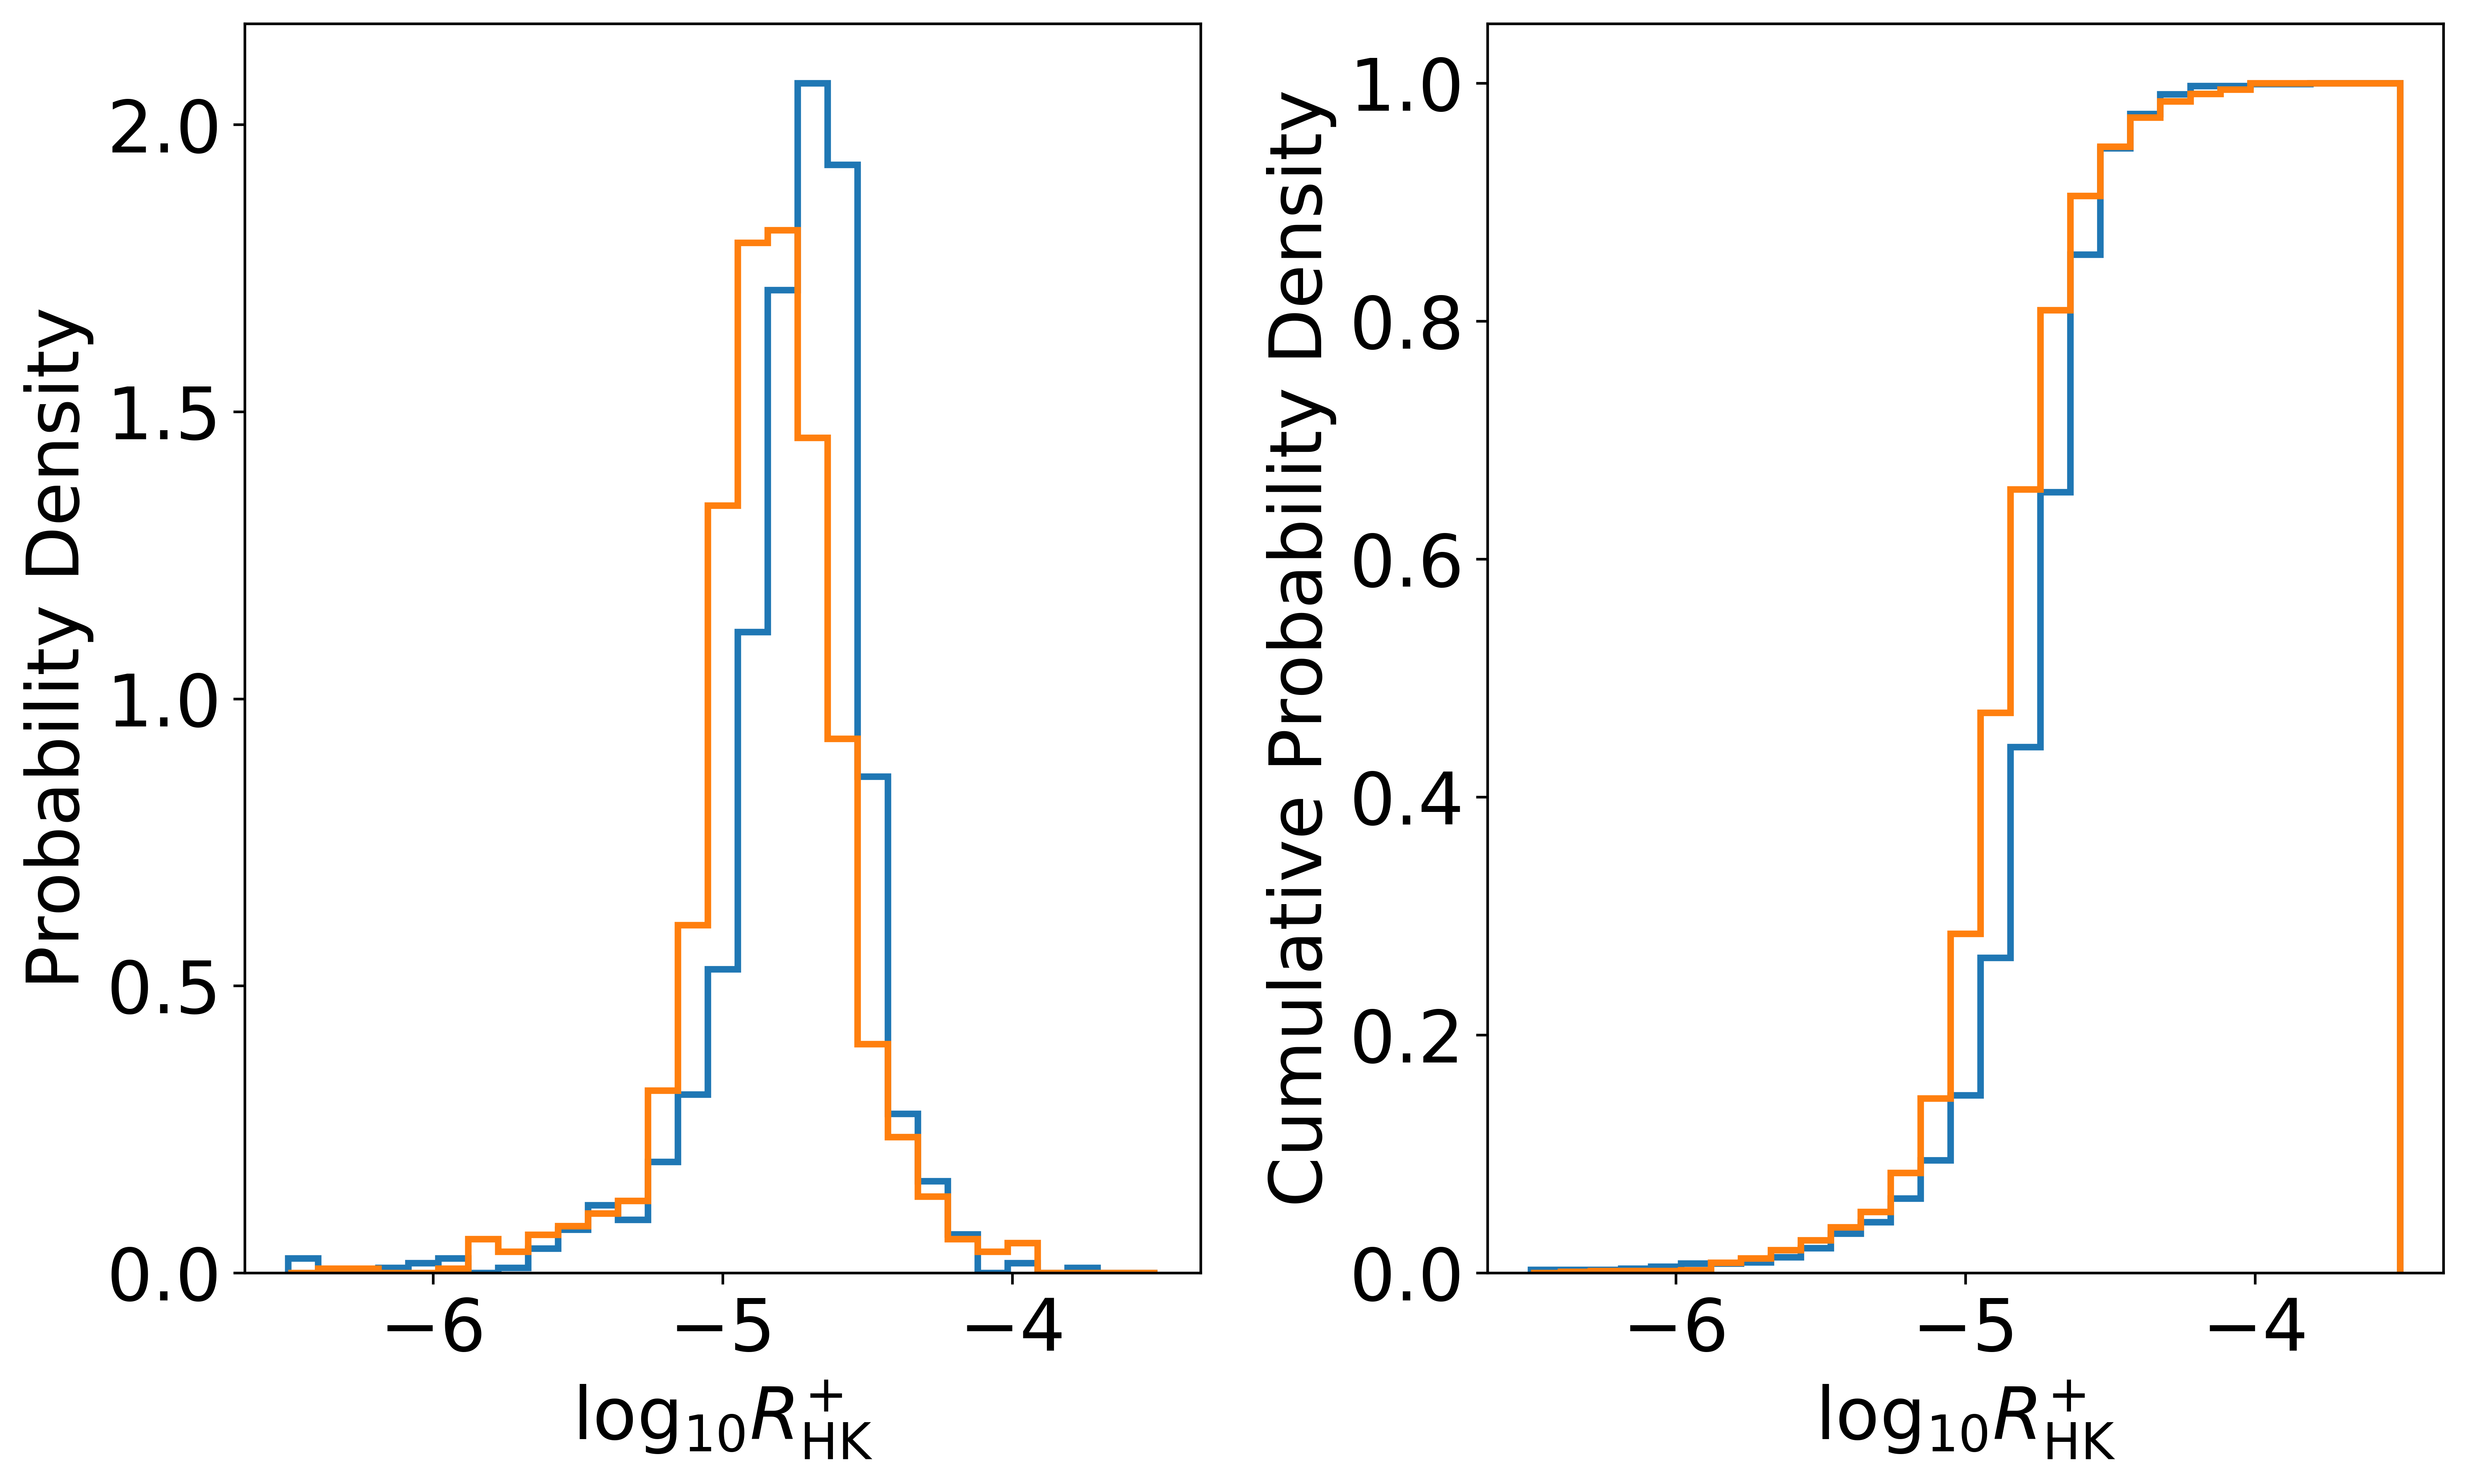
\includegraphics[width=\textwidth]{Figures/rot_gap_figures/pdf_cdf.png}
  \caption{
  	The probability density function (left) and cumulative probability density function (right) of $\log \ R^{+}_{HK}$ are separated by whether rotation was or was not detected in the close-by main-sequence LAMOST-\kepler{} crossmatch. 
	We expect less magnetically active stars to have a lower detection rate due to the decrease in prominence of stellar spots with lowering magnetic activity.
 This is supported by the data here as the non-rotation detected sample contains a larger number of low $\log \ R^{+}_{HK}$ stars.}
  \label{fig:pdf_cdf}
\end{figure}

To investigate the detectability of rotation, let us consider the fraction of targets for which we detected periods in bins of colour and $\log \ R^{+}_{HK}$.
The detection efficiency here is measured from the ratio of the number of stars with a measured rotation rate to the total number of stars in that bin.
Other works \citep[See e.g.]{claytor_recovery_2022} consider the ratio of stars with highly precise rotation period measures to those without.
We forgo any cuts to the fractional error on the rotational period as we have limited our stars to nearby stars, which should have very high precision recovery of the stellar rotation period, and we also make no cuts to the number of stars in each bin that we calculate the histogram for. 
While limiting the minimum number of stars would allow us to clarify large-scale trends, we are searching for a subsample of stars with spuriously low magnetic activity with an already small sample size.

\begin{figure}
\centering
  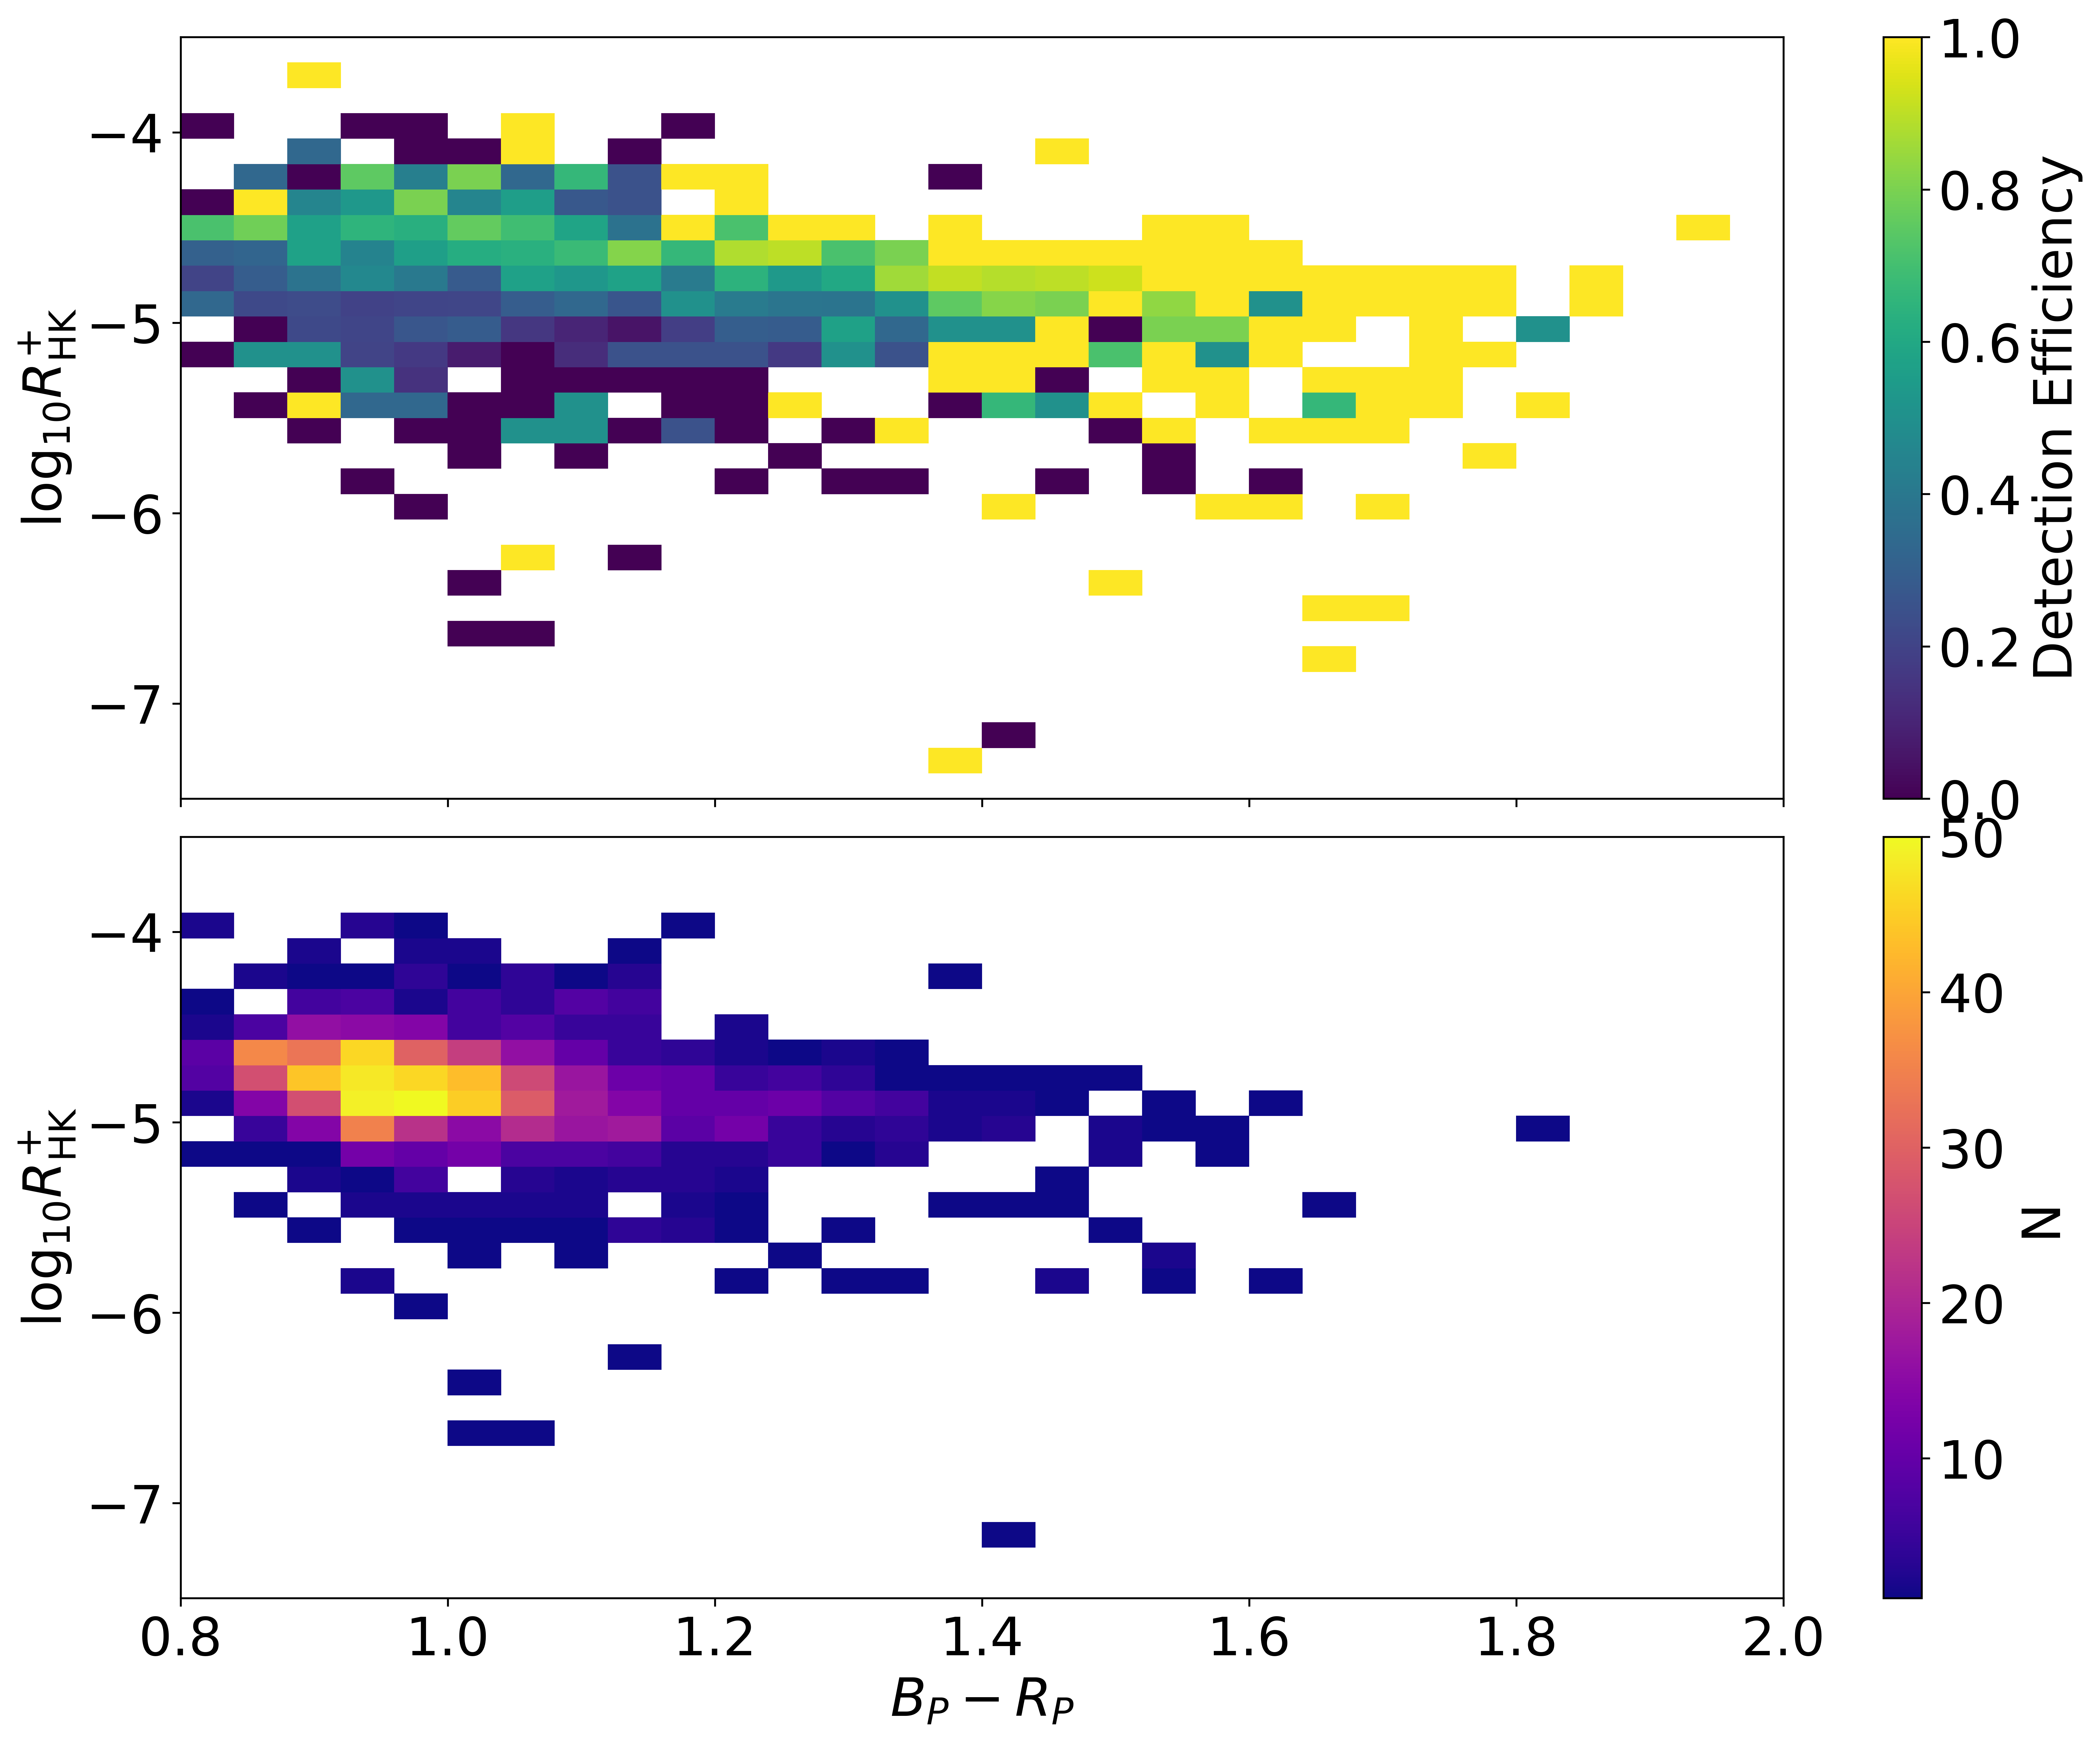
\includegraphics[width=\textwidth]{Figures/rot_gap_figures/detection_efficiency.png}
  \caption{
  	The detectability of rotation (top) and 2D histogram of stars without detected rotation periods (bottom) across \gaia{} $B_P - R_P$ colour and $\log \ R^{+}_{HK}$. 
	Rotation is preferentially measured in stars with higher magnetic activity (larger $\log \ R^{+}_{HK}$) and tends to increase with colour. Low-mass stars have a high probability of rotation being measured. Stars with low magnetic activity have a lower likelihood of rotational observation. 
Bins with detection efficiency equal to zero or one tend to contain single stars, with detected rotation or without detected rotation, respectively and are not indicative of trends in the detection efficiency.
	We do not observe an ultra-low magnetic activity population with non-detected rotation that would be required to explain the lack of observation of stars in the intermediate period gap.
	While there are stars with ultra-low $\log \ R^{+}_{HK}$ ($<$5.5) in each $B_P-R_P$ bin they can either both rotationally detected or not rotationally detected. The ultra-low magnetic activity does not indicate their lack of rotational observation probability.
}
  \label{fig:detection_efficiency_rhk}
\end{figure}

Figure \ref{fig:detection_efficiency_rhk} shows the detection fraction (top) and a 2D histogram of the non-detected rotation sub-sample (bottom) against colour and $\log \ R^{+}_{HK}$. 
We confirm that rotation is preferentially measured in stars with higher magnetic activity (larger $\log \ R^{+}_{HK}$) and tends to increase with colour. 
Low-mass stars have a high probability of rotation being measured.
If we assume that stars of the same $\log \ R^{+}_{HK}$ express the same number of stellar spots, then dimmer stars will express larger \rper{} and thus will have a higher detectability of rotation.
We do not observe an ultra-low magnetic activity population with undetected rotation that would be required to explain the lack of observation of stars in the intermediate period gap.
While there is stars with low, for a given colour bin, and ultra low $\log \ R^{+}_{HK}$ ($<$5.5) in each $B_P-R_P$ bin, stars in those bins can both be rotationally detected or not rotationally detected. 
Ultra-low magnetic activity does not indicate their lack of probability of rotational observation, and there is no subsample of ultra-low magnetic activity stars without detected rotation periods.
While stars older-slowly rotating stars also tend to have lower $\log \ R^{+}_{HK}$, which may camouflage a population of low $\log \ R^{+}_{HK}$ gap stars, they still tend to have observable rotation periods.
For the gap to exist the magnetic activity would need to drop to a point where observation of rotation period is impossible, which is not supported by the data here.

\ Section {The lack of observation of stars that could fill the intermediate period gap}
\label{sec:no_gap_stars}

For the hypothesis that the gap represents a minimum of stellar rotational period detection and that the gap is indeed full of stars, then must be enough stars without detected rotation periods to fill the shortage of observations.
In this Section, we will determine whether this is indeed the case.

We will assume that the multiple missions that have observed the rotation period gap (\kepler, \ktoo, \ZTF, \tess) missions are not biased away from observing stars within the rotation period gap and compare the distribution of stars in the \citet{mcquillan_rotation_2014} \kepler{} rotating and undetected rotating samples.
Further, this analysis will focus on very low-mass stars where the gap is most apparent - where \citet{mcquillan_rotation_2014} remains the state-of-the-art in detecting rotational periods for low-mass stars near the gap.
We make no quality cuts to the data to ensure we are not preferentially selecting for stars that could/could not possibly fill the gap.

If we compare the distribution of the number of stars in the rotation detected and undetected samples with colour, as we have shown in Figure \ref{fig:n_det_nondet}, we observe that stars with detectable rotation periods outnumber stars with undetectable rotation periods at lower masses ($B_P-R_P$ $\geq$1.3), despite the overall 3:1 ratio of the detectable rotation period to undetectable period catalogues.
In the inset of this Figure, where we compare the distributions where the gap is most apparent, we see that the proportion of stars with undetectable rotation periods to stars with detectable rotation periods decreases with decreasing mass, to a minimum of 1:10 undetectable to detectable rotation periods at the lowest masses.
This suggests that there are not a large number of stars available to fill the rotational period gap.

\begin{figure}
\centering
  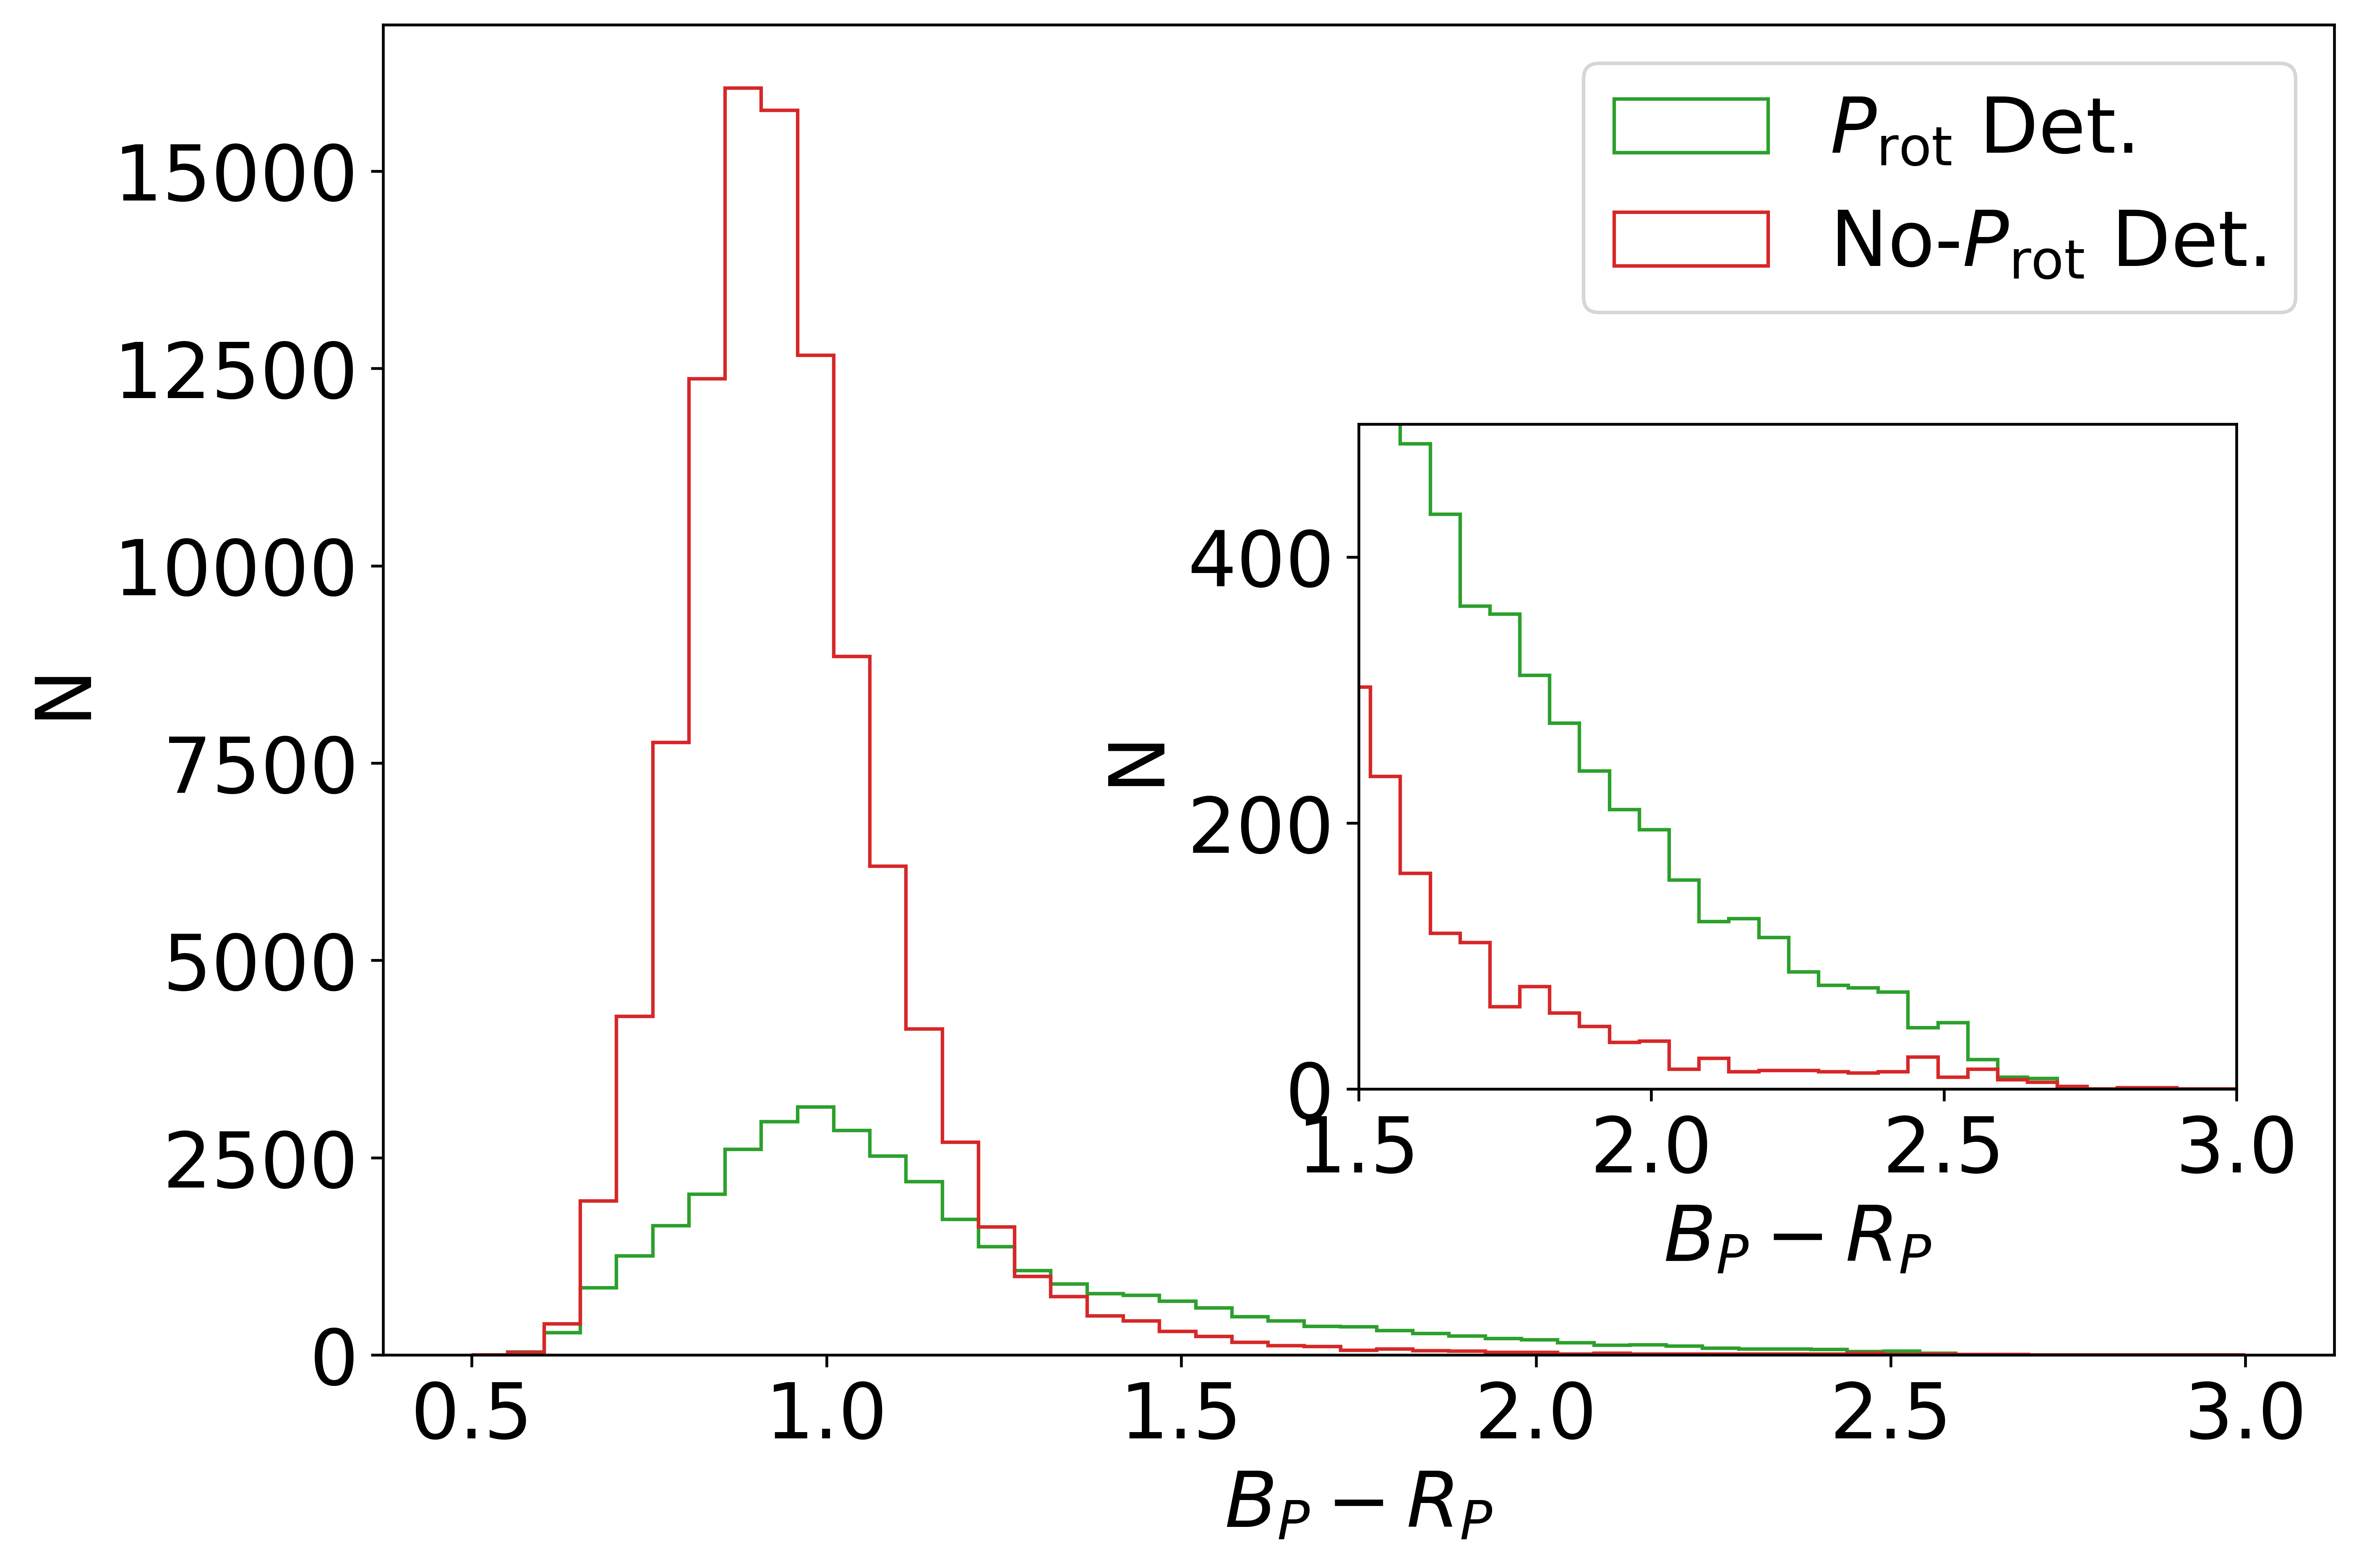
\includegraphics[width=\textwidth]{Figures/rot_gap_figures/hist_obs.png}
  \caption{A histogram of the distribution of $B_P-R_P$ colour of stars with (green) and without (red) detected rotation periods. \textbf{Inset:} A zoom-in of the distribution for $B_P-R_P\geq1.5$ where the rotational period gap is most apparent. The distribution in colour of stars with and without detected rotation periods vary. The undetected rotation sample is strongly biased towards stars with $B_P-R_P$ close to 1, comparative to the lower-mass stars where the number of stars drops quickly. Despite the $\sim$3:1 ratio of the number of stars with undetected rotation periods to those with detected rotation periods, the number of stars without detected rotation periods drops below those with detected rotation at $B_P-R_P\geq1.3$.
  	}
  \label{fig:n_det_nondet}
\end{figure}

We will more concretely investigate this by determining how many stars would be required to fill the gap - or rather for the dearth in observations to be undetectable in the low mass range where the proportion of stars between the samples is largest and where the gap is most apparent ($B_P-R_P$ $\geq$1.5).
To find the number of stars required for the dearth of observations to be no longer considered a dearth we first separate the sample with detected rotation into bins of $B_P - R_P$  from 1.5-2.2 of size 0.045 (15 bins).
In each colour interval, we then split the data into log rotational period intervals of width 0.07 dex between 1.0 and 1.7 dex (10 bins) - which correspond to 10 and 50 days, respectively.
We then calculate the number of stars in each slice of log period for a given colour range.
In Figure \ref{fig:n_col} we show the number of stars in each slice (scatter points) against $\log_{10}$ of the rotation period for each colour range indicated in brackets to which we have fit a cubic spline (dashed)
From the cubic spline, we determine the position of the local minima in number of stars with detected rotation period, which is indicated by the solid vertical black line.
The calculation of the position of the minima is again an automated process as carried out in the previous Sections.
To calculate the number of stars required for the dearth, we compare the average of the two scatter bins surrounding the closest bin of the minima position.
While this approach is admittedly naive, as it assumes all of the stars will be in the bin closest to the minima rather than being distributed throughout the dearth region, it places a lower bound on the stars required to fill the gap.

\begin{figure}
\centering
  \includegraphics[width=\textwidth]{Figures/rot_gap_figures/n_col.png}
  \caption{
  	Number of stars in each bin against $\log_{10}$ of the rotation period in bins of colour \gaia{} $B_P-R_P$ (indicated in brackets). Here we have fitted a cubic spline to the number of stars in each bin and calculated minima using the first and second derivatives of the fitted cubic spline. Solid vertical black lines show the minima in number of stars. These minima are the rotational period gap.
}
  \label{fig:n_col}
\end{figure}

In Figure \ref{fig:stars_not_fill} we compare the number of stars required to fill the gap to the number of stars without detected rotation periods in each colour range.
The number of stars required to fill the gap is approximately constant at N $\sim$ 20.
This suggests that the number of stars required gap is independent of the total number of stars observed in that mass range.
Suppose the gap is full of stars without detectable rotation periods.
In that case, we expect the proportion of stars required to fill the gap to increase proportionate to the total number of stars (detected and non-detected rotation), but this is not the case.
The number of stars required to fill the gap is much smaller than the number of stars without detected rotation periods for $B_P-R_P<1.8$. 
Still, as colour increases and the number of observed (detected rotation period stars) stars decrease, the number of stars required to fill the gap becomes the majority of stars without detected rotation periods.
This suggests that for the gap to be full of stars with undetected rotational period stars, all of the stars in the undetected rotational period sample would need to be in this small rotational period range, and only a very small number of stars with undetected rotation are the result of noise or inclination effects.
The requirement of most (if not all) stars within the undetected rotation period sample suggests that the gap is not full of stars with undetectable rotation.

\begin{figure}
\centering
  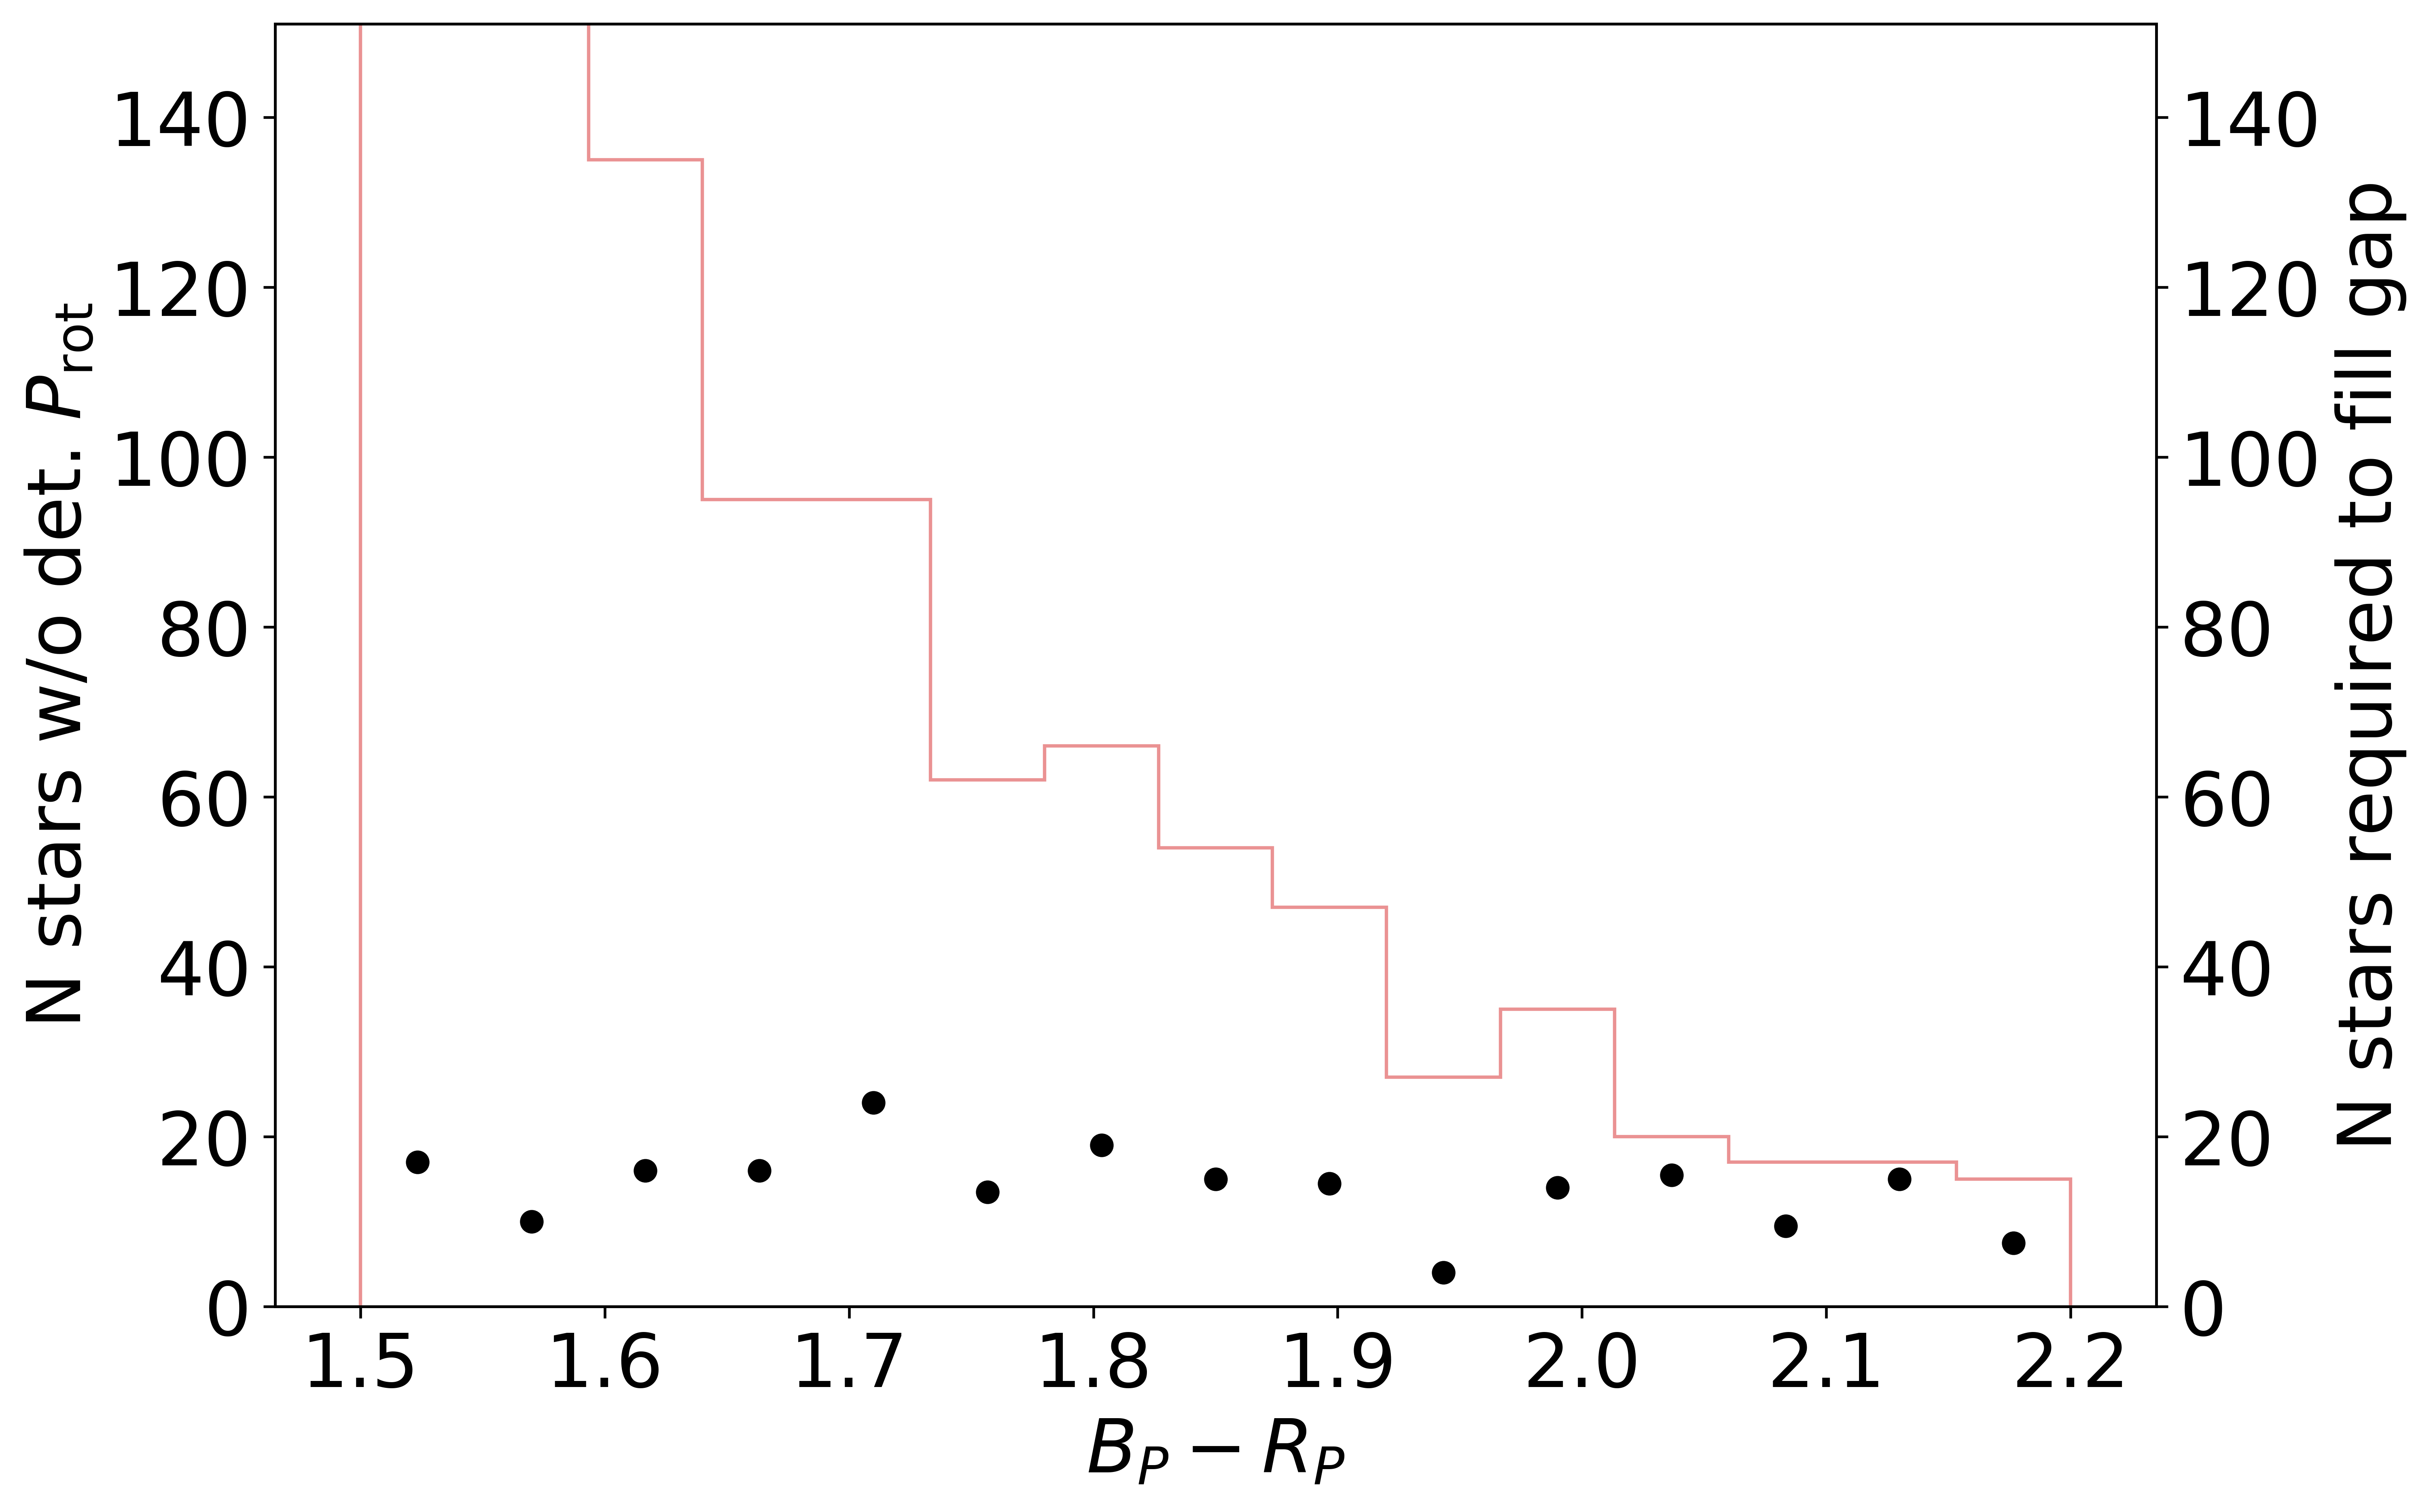
\includegraphics[width=\textwidth]{Figures/rot_gap_figures/stars_donot_fullgap.png}
  \caption{
  	The number of stars required to fill the gap (black scatter points) against the number of stars with undetected rotation periods against $B_P-R_P$. The number of stars required to fill the intermediate period gap is roughly constant at N $\sim$ 20. While the number of stars without detected rotation greatly outnumbers the number required to fill the gap below $B_P-R_P \sim 1.8$, the two are almost equal for lower mass stars.
}
  \label{fig:stars_not_fill}
\end{figure}


\section{Latitudinal differential rotation}
\label{sec:lat_diff_rot}

We have proposed in this work that there is a lack of evidence to suggest that the rotational period gap represents a regime of evolution by which stars have low detectability due to low stellar activity.
The only other proposed mechanism to explain the gap arises from extreme wind braking, causing stars to spin down quickly across the gap.
Leaving that explanation for the coming Section, we propose a previously uninvoked mechanism to consider: the onset of latitudinal differential rotation.
Stars, most concretely for the Sun, have been observed to express latitudinal differential rotation.
Further, stars express latitudinally distributed spots across their surface.
The observed rotation rate of stars from stellar spots is generally taken as the average rotation rate across the surface of a star \citet{santos_surface_2021}.
If a star swiftly transitioned from flat to latitudinally differentially rotating, then the observed average rotation rate could change significantly.

\citet{benomar_nearly_2015, benomar_asteroseismic_2018, bazot_latitudinal_2019, hall_weakened_2021}, for example, have measured the differential rotation of main-sequence solar-like, in terms of mass and rotation rate, stars through asteroseismology.
Within their sample \citet{bazot_latitudinal_2019} found that every star in their sample expressed evidence of latitudinal differential rotation that is equator-fast (colloquially known as solar-like).
\citet{saar_starspots_2011} performed observations of the latitudinal differential rotation of single main-sequence stars from Ca II HK $P_{\rm{rot}}$ variations \citep[e.g.]{donahue_relationship_1996} and photometric $P_{\rm{rot}}$ variations \citep[e.g.]{messina_magnetic_2003}.
They found that fast-rotating stars ($R_o < 0.45$) support quenched - latitudinally flat \footnote{or rather, close to latitudinally flat} - rotation profiles, which increase in scale of differential rotation, which they measure as the rotation rate difference between the equator and at a latitude of 60$^{\circ}$, proportional to the Rossby number 
\begin{equation}
\frac{|\rm{d}\Omega|}{\Omega} \propto R_o^2
\end{equation}
Intermediate rotating stars $0.45\leq R_o \leq 2$ support solar-like (equator fast) differential rotation and slow rotators ($R_o\geq2$) support anti-solar (pole fast) rotation.
They argue that in both of these regimes, the scale of differential rotation is constant - $\frac{|\rm{d}\Omega|}{\Omega} \sim 0.2$ - but that the sign of the differential rotation changes suddenly at $R_o \sim 2$.
\citet{brun_powering_2022} showed, through 2-D magnetohydrodynamic simulations, that the presence of a magnetic field inhibits the growth of differential rotation for fast rotators.
They suggest that the growth of differential rotation for fast rotators could scale with $\frac{|\rm{d}\Omega|}{\Omega} \propto R_o^p$, where $p$ could take any value between 2 and 6.
They also tentatively argue for the growth of the scale of differential rotation for anti-solar rotators proportional to the square of the Rossby number.

Interestingly the transition from latitudinally flat rotation profiles, to equator fast rotation profiles occurs near $R_o \sim 0.5$ - the Rossby number where the rotational period gap occurs.
If latitudinal differential rotation becomes significant at this point in the evolution of rotation of a star, then the rotation period gap may reflect a sudden increase in average, and thus observed, surface rotation period from that onset.
We consider this as the mechanism underlying the intermediate period gap by investigating an observationally motivated observed rotation period distribution under the proposed differential rotation relationships proposed by \citet{saar_starspots_2011} and \citet{brun_powering_2022}

%Well below the gap, stars have a latitudinally flat rotation profile \cite{}.
%As their cores and envelopes recouple the surface continues to spin down and lose angular momentum through wind braking.
%To counteract this loss of angular momentum at the equator, angular momentum transport occurs latitudinally towards the equator slowing the spin-down of the equator rotation rate but in turn, inducing an equator-fast latitudinal differential rotation profile.
%The latitudinal differential rotation grows swiftly, and the average observed rotation rates of stars drop as a result.
%The swift onset of this differential rotation leads to only a small number of stars being observed with rotation rates that place them within the gap.

We generate 40,000 main-sequence and early post-main-sequence stars with various values of mass, age, metallicity and rotations rate.
We drew masses from a uniform mass function between 0.5 and 1. 
This limits our range of masses to those with a radiative surface and convective core and especially targets stars where the rotational period gap is most apparent. 
We have not assumed an initial mass function here - this is because the \kepler{} sample is biased towards brighter high-mass stars, which we assume here effectively cancels out, say, a Saltpeter IMFs bias towards a larger number of low-mass stars.

Metallicity is drawn from a distribution to approximately reflect what is observed in the Milky Way. Specifically, we defined a variable $\phi$ to be drawn from a Beta distribution
\begin{equation}
  \phi \sim \mathcal{B}\left(\alpha=10, \beta=2\right)
\end{equation}
and applied a transform from $\phi$ to [Fe/H] by requiring the metallicities be bounded between $[\mathrm{Fe/H}]_\mathrm{min} =-2$ and $[\mathrm{Fe/H}]_\mathrm{max} = +0.5$. We also required that the mode of $\phi$, defined as $\frac{\alpha - 1}{\alpha + \beta - 2}$ for a Beta distribution, occurs at Solar metallicity. This leads to the transform:
\begin{equation}
  [\mathrm{Fe/H}] = \left(\frac{}{}[\mathrm{Fe/H}]_\mathrm{max}-[\mathrm{Fe/H}]_\mathrm{min}\right)\left(\phi - \frac{\alpha - 1}{\alpha + \beta - 2}\right) \quad .
\end{equation}

The stars we generate mock data for in this work span from the zero-age main sequence (ZAMS) to low-luminosity subgiants. We draw equivalent evolutionary phase (EEP) values from a uniform distribution EEP $\sim \mathcal{U}(200,450)$, where $\mathcal{U}\left(x,y\right)$ denotes a uniform prior between x and y.
The bounds of this range (200 and 450) represent the ZAMS and the low-luminosity subgiant phase, respectively. 
Using the EEP, mass and metallicity, we interpolate a position along the MIST stellar isochrones \citep{morton_isochrones_2015} to calculate the expected \teff and \logg for each star.
We also obtain the star's age (post-ZAMS) that we can use in conjunction with the other stellar parameters to determine rotational properties (see below). We have limited the age of the stars we consider in this work up to the age of the Sun. 
This is the range available for rotational rate.
The equator surface rotation period is interpolated from stellar cluster-tuned rotational isochrones given the stellar age and mass (Table A1 in \citet{spada_angular_2016}).
This sample does not produce the observed rotational period gap and assumes a smooth distribution of rotational periods around the $R_o =0.5$.

We evaluate the first evaluate the convective turnover timescale ($\tau_c^{\rm{CS}}$) of our sample using the scaling relation derived in \citet{cranmer_testing_2011},
\begin{equation}
	\tau_c^{\rm{CS}} = 314.24 \ \exp\left[ -\frac{T_{\rm{eff}}}{1952.5\rm{K}} - \left( \frac{T_{\rm{eff}}}{6250 \rm{K}}\right)^{18}\right] + 0.002 d
\end{equation}
from this we calculate $R_o$ of our sample from $R_o = P_{\rm{rot}}/\tau_c^{\rm{CS}}$.

From $R_o$ we obtain the scale of differential rotation of our stars.
We adopt the 3 different piecewise functions to represent the evolution of the scale of differential rotation between the equator and at a latitude of 60$^{\circ}$.
The first is the observational trend found in \citet{saar_starspots_2011}, where the scale of differential rotation grows with a decrease in rotation rate below $R_o\leq0.5$ and is constant above this limit,
{\centering
$\frac{|\Delta\Omega|}{\Omega} = \left\{
\begin{array}{ll}
   0.2/(0.45^{2.5}) R_o^{2.5}& R_o\leq 0.45 \\
   0.2 & 0.4 \leq R_o
\end{array} 
\right\}$\par}
where we have ensured continuity with the prefactor $0.2 \ / 0.45^{p}$, and $\Delta \Omega$ is the difference between the equator rotation rate and the rotation rate at a latitude of 60$^{\circ}$.
The other two relations we adopt reflect two cases for the transition of the scale of differential rotation that are steeper than the \citet{saar_starspots_2011} relation that fall within the range suggested by the edges of the scale of differential rotation in \citet{brun_powering_2022} (See Figure 8 in their work).
These are:
{\centering
$\frac{|\Delta\Omega|}{\Omega} = \left\{
\begin{array}{ll}
   0.2/(0.45^4) R_o^4& R_o\leq 0.45 \\
   0.2 & 0.45\leq R_o\leq 2 \\
   0.2/(2^2) R_o^2& 2\leq R_o \\
\end{array} 
\right\}$\par}


and

{\centering
$\frac{|\Delta\Omega|}{\Omega} =  \left\{
\begin{array}{ll}
   0.2(0.5^6) R_o^6& R_o\leq 0.45 \\
   0.2 & 0.45\leq R_o\leq 2 \\
   0.2/(2^2) R_o^2 & 2\leq R_o \\
\end{array} 
\right\}$\par}

where the prefactors $0.2 \ / \ 0.45^{4}$, $0.2 \ / \ 2^{4}$, $0.2 \ / \ 0.45^{6}$, and $0.2 \ / \ 2^{2}$ ensure continuity.
We have chosen these two relations to investigate the effect of the steepness of the relation between differential rotation and $R_o$ on the observed rotational period distribution as well as the effect of an increase to the scale of differential rotation beyond $R_o = 2$.
The relations we investigate in this work are shown in Figure \ref{fig:compar_diff_rot}, where we show the relation determined in \citet{saar_starspots_2011} (orange), the range of the scale of differential rotation suggested by \citet{brun_powering_2022} and the two steeper relations (green and purple respectively) relations we adopt in this work.

Here we assume that have solar-like differential rotation profile below $R_o = 2$ - the sign of $\frac{\Delta \Omega}{\Omega}$ is positive - and above this $R_o$ the star instantly transitions to anti-solar like - the sign becomes negative. 
From this, we calculate the differential rotation by multiplying this factor by the equator rotation rate.
While the instantaneous nature of this transformation may not be physical, the transition from solar-like to anti-solar-like differential rotation will have the same effect - an increase in the density of stars with observed rotational periods near the transition.

We adopt a second-order solar-like differential rotation profile with the rotation rate with inclination:
\begin{equation}
    \Omega\left(\theta\right) = \Omega_{\rm{eq}} + \frac{\Delta \Omega}{\sin^{2}\left(60^{\circ}\right)} \sin^2{\theta}
\end{equation}
where the prefactor $\frac{\Delta \Omega}{\sin^{2}\left(60^{\circ}\right)}$ ensures continuity.

We can then calculate the average observed rotation rate from the integral of the rotation rate given a distribution of stellar spots on a star's surface divided by the star's surface area, both calculated where the stellar spots are expressed.
Here we are assuming that all stars in our sample are viewed equator-on.
While this is not the case for all stars, the rotational period gap is not an effect of the observation angle.
Further, inclination angles are uniformly distributed in $\cos{i}$, and stars must be viewed close to the equator for their rotation periods to be measurable (see Section \ref{sec:intro}) - therefore, most stars with observed rotation profile are close to equator-on.

The distribution of stellar spots on the surfaces of these stars requires some thought.
While the probability distribution of stellar spots of the Sun is well known, this distribution does not account for the variation of the distribution of spots with mass, equator rotation rate or differential rotation.
 \citet{granzer_spotted_2003} performed magnetohydrodynamic simulations of rotating low-mass stars in the Pleiades and determined the distribution of stellar spots of stars of various masses and rotation rates (see Figure 3. in their work).
We adapt their findings to suit the work we complete here.
We take the sparse grid of grid of equator rotation rates and stellar masses and measure the maximum and minimum latitudes that stellar spots are expressed for those models.
 In this work, we assume that stellar spots are uniformly distributed between the maximum and minimum latitudes that stellar spots are expressed.
 While their work explicitly contradicts this assumption, their distributions are decidedly non-uniform, their grid is sparse, and we cannot easily interpolate between distributions of stellar spots.
 Furthermore, the stellar spot distributions can be skewed towards the equator and the pole, dependent on the mass and rotation rate of the model - any shape of the distribution that we assume does not adequately reflect the presented stellar spot distributions in their work.

If the stellar spots are uniformly distributed, then the average rotation rate of the surface is simply the average rotation rate between the edges of the latitudes where the stellar spots are expressed.
The average rotation rate is calculated from the integral of the rotation rate divided by the surface area both over the maximum and minimum latitudes that the spots are expressed,
\begin{equation}
	\Omega_{\rm{avg}} = \int^{\theta_{\rm{max}}}_{\theta_{\rm{min}}} \Omega(\theta) \sin(\theta) \rm{d}\theta \ / \  \int^{\theta_{\rm{max}}}_{\theta_{\rm{min}}} \sin(\theta) \rm{d}\theta
\end{equation}
where rotation rate is independent of radius and azimuthal angle, and their contributions cancel.
Here $\theta_{\rm{max}}$ and $\theta_{\rm{min}}$ are the upper and lower bounds of the distribution of spots on the surface of the star.
Because the rotation profile is symmetric about the equator of rotation we only need to calculate the contribution to the rotation rate in one hemisphere.

We compare the effect of each of the chosen relations between differential rotation and $R_o$ on the observed rotation period of $0.7 M_{\odot}$ star in Figure \ref{fig:comp_per}.
The growth of differential rotation below $R_o<0.45$ is observed at $P_{\rm{rot, injected}}$ < 20 d.
Steeper relations of $R_o$ with differential rotation in this range result in a quicker growth in observed rotation periods for the same injected period.
The steeper the growth of the observed rotational period, the lower the number of stars that would be observed with that rotational period, while the transition from solar-like to anti-solar-like rotation ($P_{\rm{rot, injected}}$ = 70 d) results in an instantaneous transition from observed rotational periods greater than the injected value, to an observed rotational period less than the injected value.

Under these assumptions, the observed rotation period under each relation of differential rotation and $R_o$ of the stars in our synthetic sample can be calculated.
The resulting distributions of stars (blue, orange, green and purple) relative to the observed distribution of \kepler{} rotational periods measured in \citet{mcquillan_rotation_2014} (black) are shown in Figure \ref{fig:comp_dist}.
Here, the colour of each distribution corresponds to the same colour showing the relation between differential rotation and $R_o$ in Figure \ref{fig:compar_diffrot} and blue corresponds to the injected, or flat rotation profile observed, rotational period.
For clarity, we have also shown the 2D histograms of the distributions in Figure \ref{fig:comp_hist} where the effects are more recognisable.

Comparing the rotational distributions under these differential rotation relations, we observe that a dearth of observations occurs when a transition from latitudinally flat to solar-like differential rotation at $R_o = 0.45$ is introduced to calculate the observed rotation rate of stars.
Further, the increased density of observation of stars above the intermediate period gap in the \kepler{} sample is reproduced under this model - unlike a model of extreme magnetic braking to explain the gap.
The distinctness, or rather the decrease in density of stars within the gap, increases with the power on $R_o\leq 0.45$.
However, the decreased density of stars within the gap is, qualitatively, most accurately reflected by the observationally prescribed relation between $R_o$ and scale of differential rotation found in \citet{saar_starspots_2011}.

We also find an over-density of stars where the transition from solar-like to anti-solar-like latitudinal differential rotation occurs ($\log P_{\rm{rot}} = 1.2$, $T_{\rm{eff}} = 6000K$).
While the observed \kepler{} rotation periods do contain a high density of stars near this location, we are hesitant to suggest whether this feature is the result of this transition or from the selection function of \kepler{} observations being biased towards higher mass, brighter, stars.
Further, given the small number of nearby, old ($\geq$3 Gyr) clusters in the \kepler{} field, and the evolution of rotational spin-down with variations to the latitudinal differential rotation, we believe that the cluster-tuned isochrones used in this work to determine the rotational periods of stars are less reliable for these stars.

\begin{figure}
\centering
  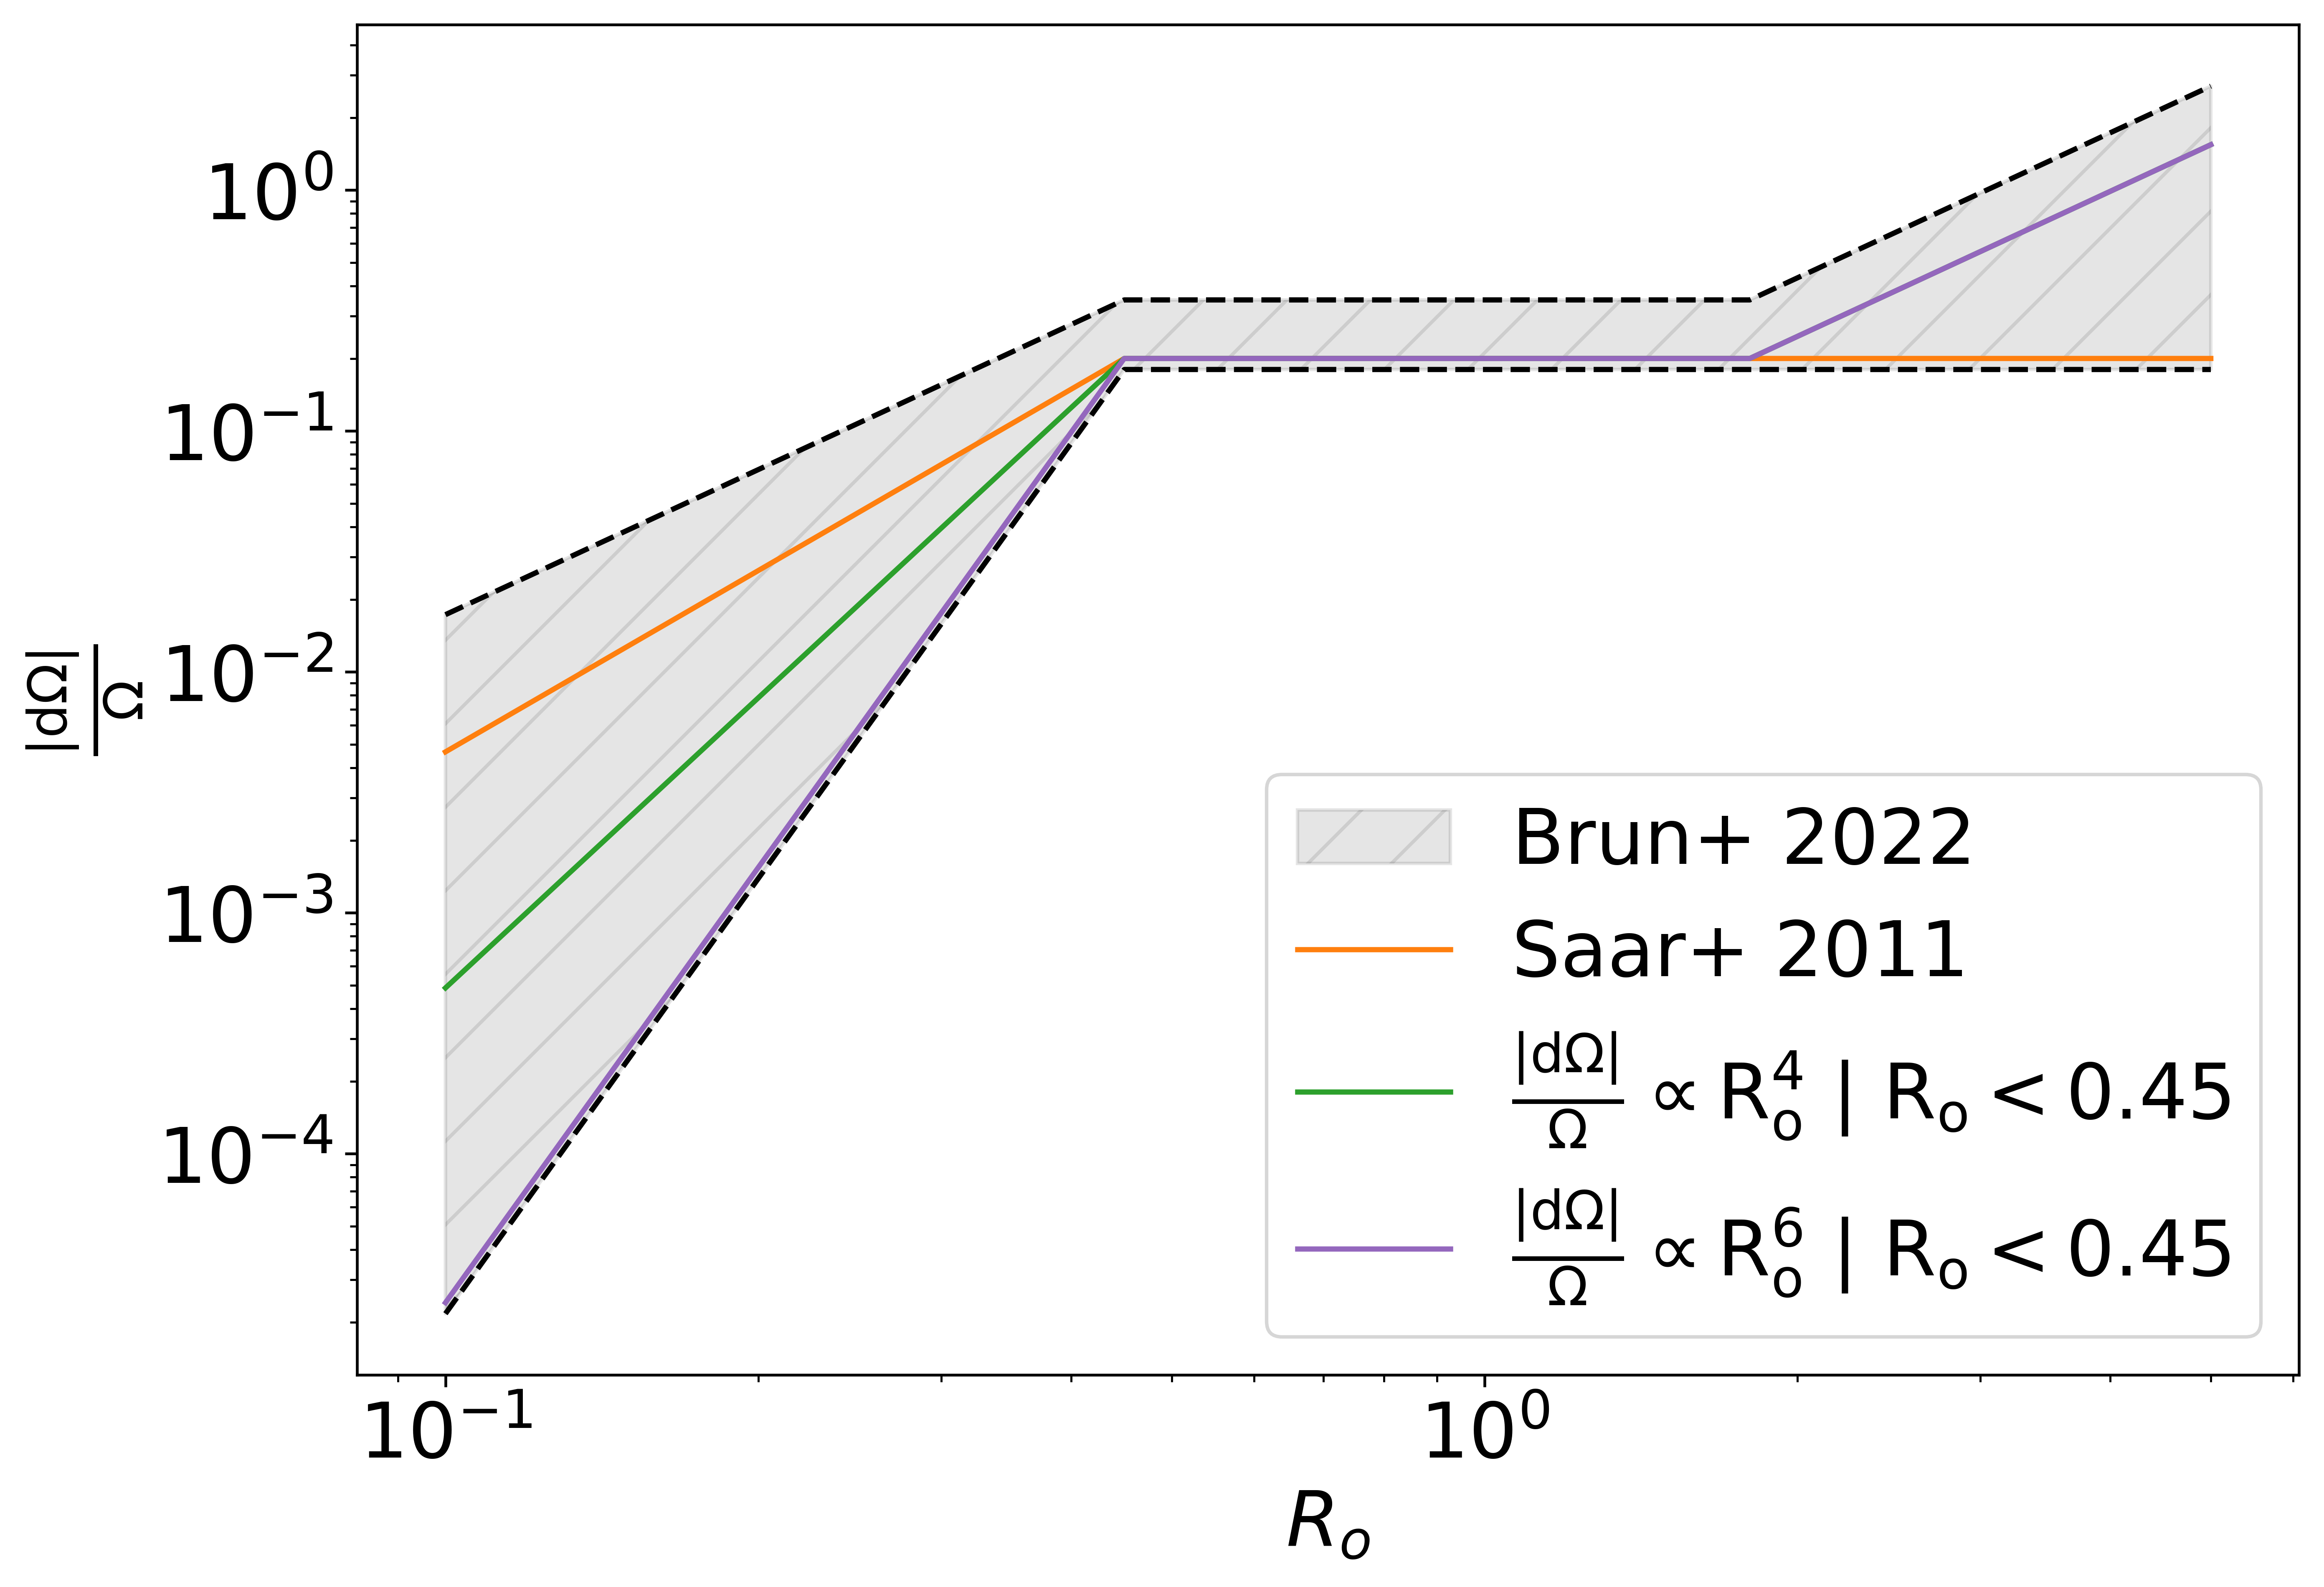
\includegraphics[width=\textwidth]{Figures/rot_gap_figures/comparison_diffrot.png}
  \caption{
  	The various relationships between latitudinal differential rotation and the stellar $R_o$ adopted in this work. We compare between the observationally derived relation from \citet{saar_starspots_2011} (orange) and two steeper relations for $R_o\leq0.45$, $|\Delta \Omega|/\Omega \propto R_o^4$ (green) and $|\Delta \Omega|/\Omega \propto R_o^6$ (purple). The scale of differential rotation is greater for the latter two relations and we have an increase to the scale of differential rotation for $R_o\geq2$. All three relations are consistent with the magnetohydrodynamic investigations into stellar differential rotation from \citet{brun_powering_2022}.
}
  \label{fig:compar_diffrot}
\end{figure}

\begin{figure}
\centering
  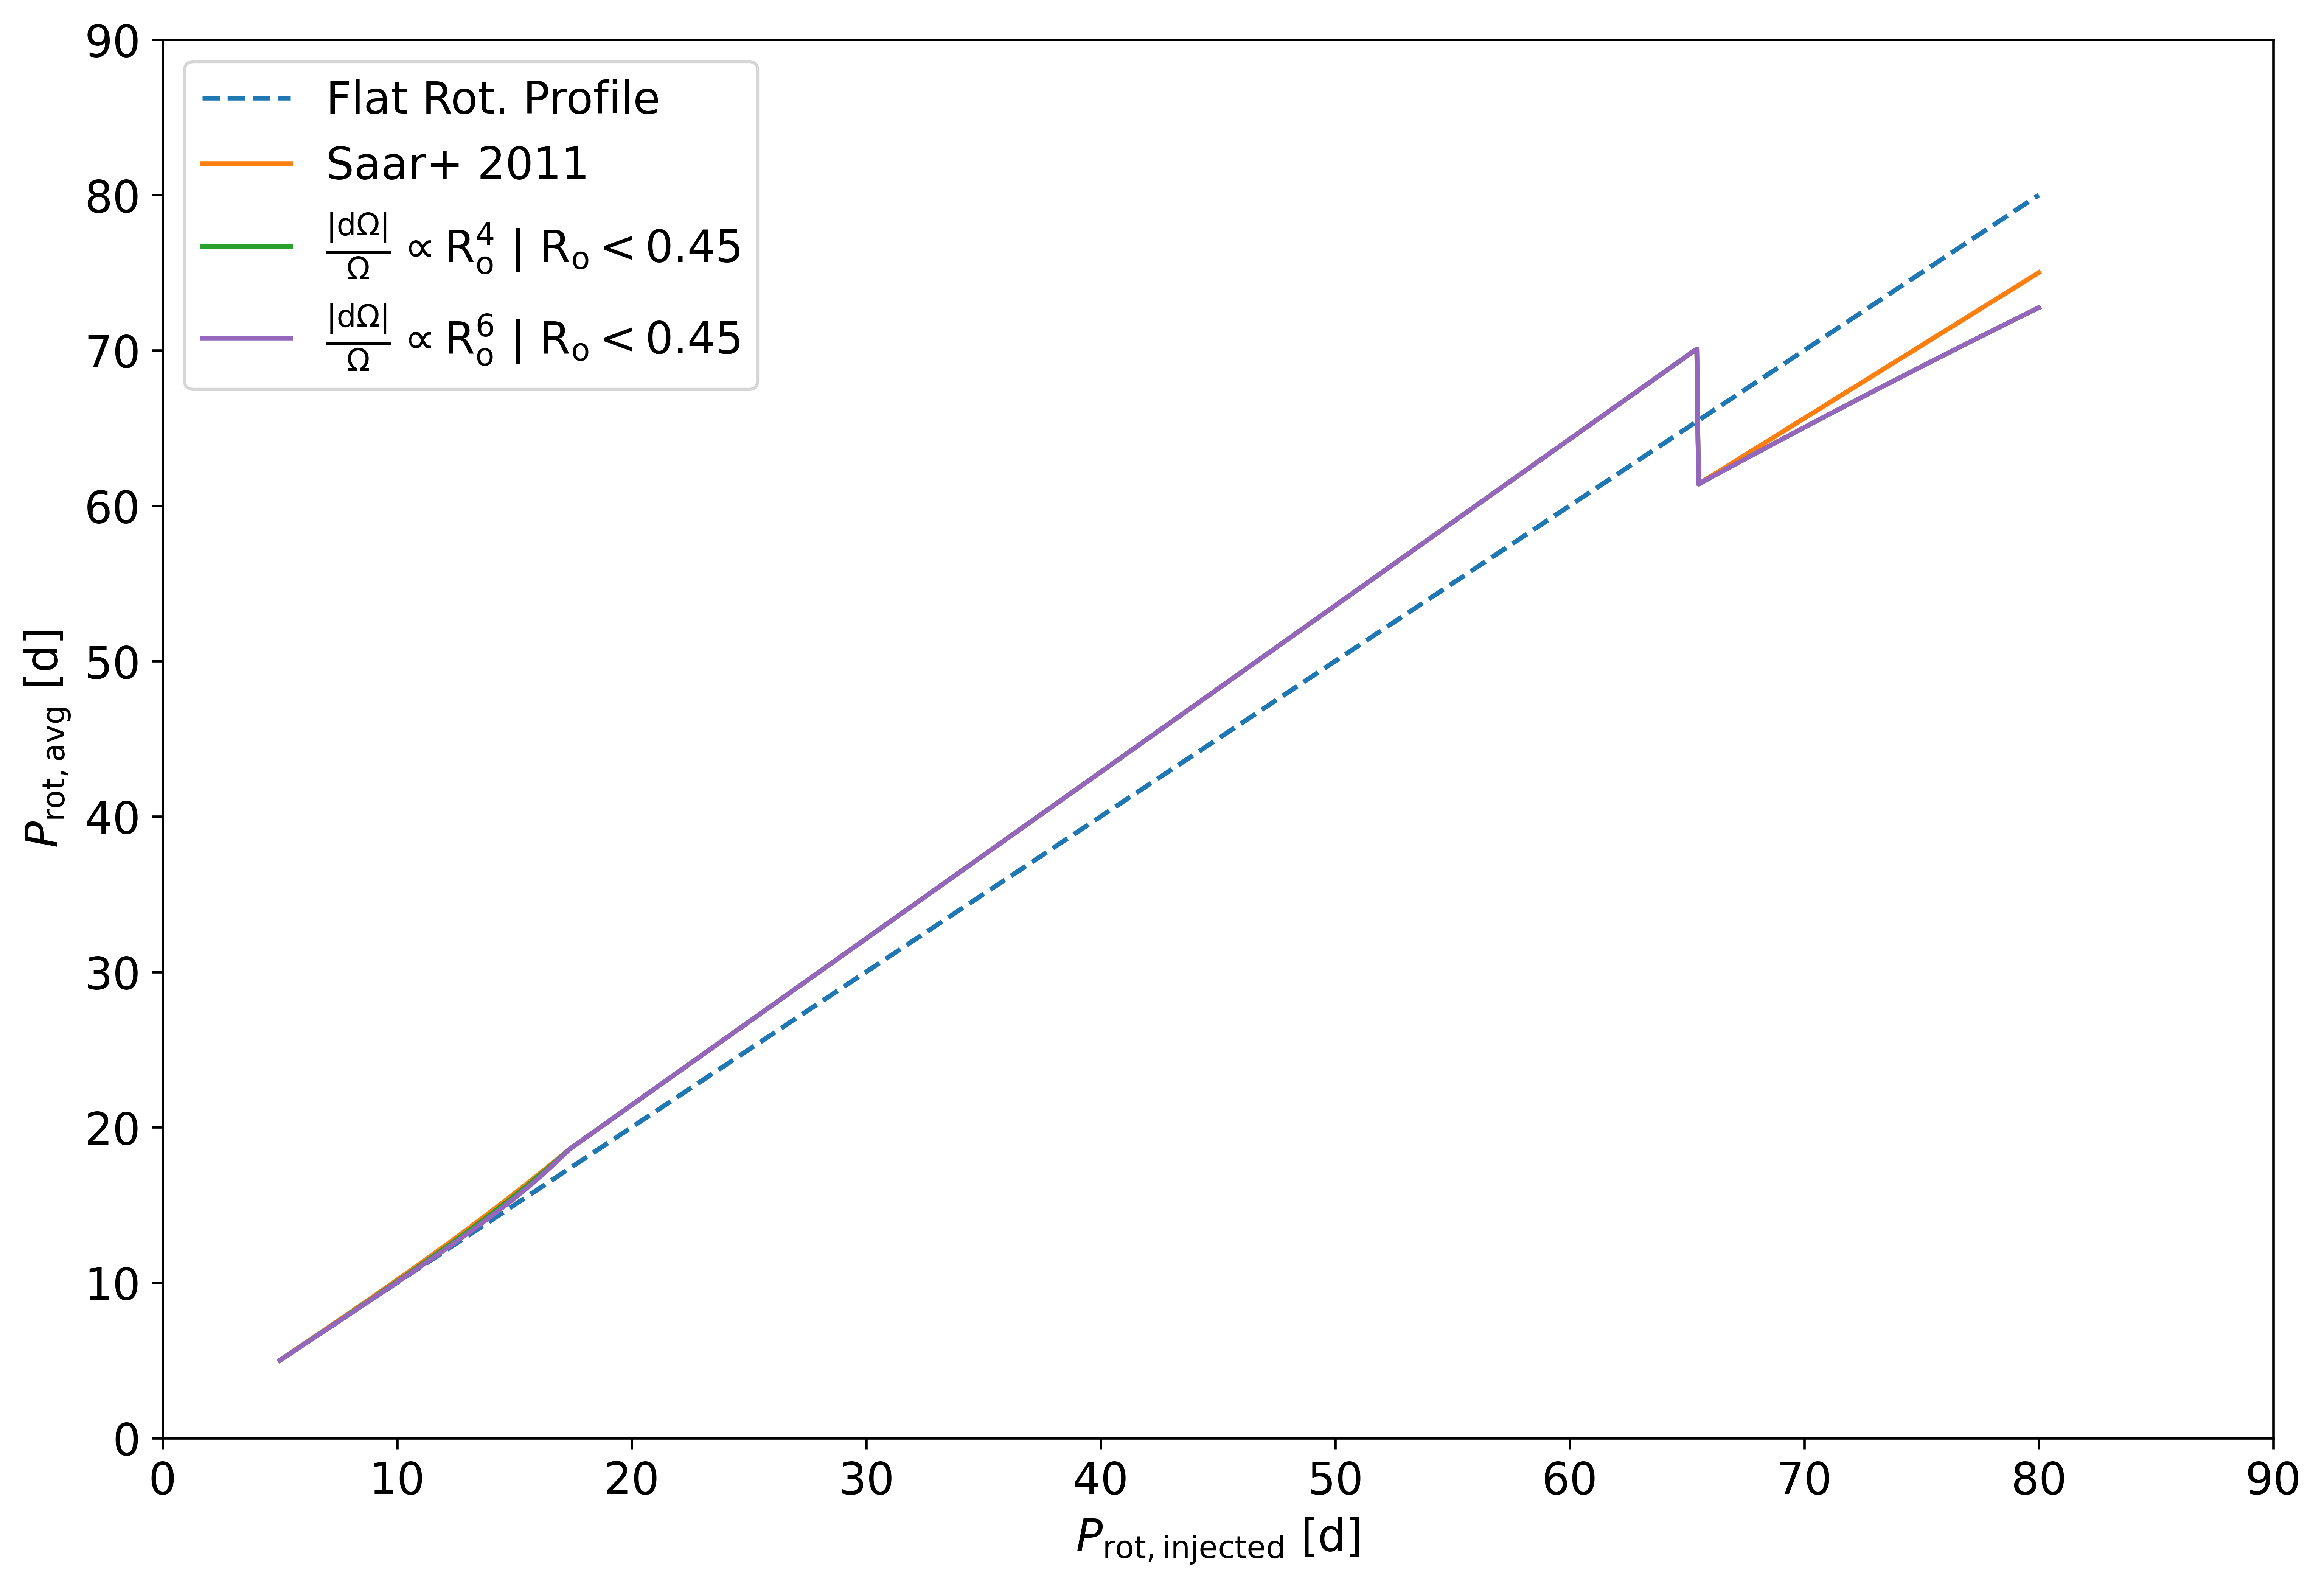
\includegraphics[width=\textwidth]{Figures/rot_gap_figures/comparison_observed_rot_periods.png}
  \caption{
  	The effect of the differential rotation on the observed rotational period of a 0.7 $M_{\odot}$ star. Here the colour of the relations corresponds to the adopted differential rotation relation in Figure \ref{fig:compar_diffrot} compared to the observed rotation profile of a latitudinally flat rotating star. At $R_o<0.45$ for injected rotation periods ($P_{\rm{rot, injected}}$) less than 20 days. It is evident that steeper relations between $R_o$ and differential rotation lead to more rapid growth in observed rotation periods for the same injected period. Moreover, a steeper growth in the observed rotational period corresponds to a lower number of observed stars with that particular rotation period. The transition from solar-like to anti-solar-like rotation, occurring at $P_{\rm{rot, injected}}$ = 70 days, results in an instantaneous shift in observed rotational periods from being greater than the injected value to being less than the injected value.
}
  \label{fig:comp_per}
\end{figure}

\begin{figure}
\centering
  \includegraphics[width=\textwidth]{Figures/rot_gap_figures/comp_dist.png}
  \caption{
  	The observed rotational period distributions of the synthetic sample of stars given various relations between latitudinal differential rotation and $R_o$ overlayed over the observed distribution of rotational periods of the \kepler{} sample from \citet{mcquillan_rotation_2014} (black). Here, the coloured observed rotational period distributions correspond to the various differential rotation relations adopted in this work, as seen in Figure \ref{fig:compar_diffrot}. The latitudinally flat (blue, top left) sample reflects the injected rotational periods of our sample considered in this work. We observe that there is no intermediate period gap in this synthetic sample of stars without differential rotation. If we include the effects of differential rotation on the observed rotation period, a dearth of observations at the transition between latitudinally flat ($R_o<0.45$) and solar-like rotation occurs precisely at the location of the intermediate period gap. 
 Further, we find that as the steepness of the relation between $|\Delta \Omega| / \Omega$ increases (where in order of increasing steepness, we have the orange, green and purple distributions) the gap becomes more distinct - fewer stars are observed within the gap. We also find that due to the transition from solar-like to anti-solar-like differential rotation, we obtain an over-density of stars consistent with the overdensity of slow-rotating stars near 6000K. See \ref{fig:comp_fig} for 2D histograms of the distribution of rotation periods in these panels.}
  \label{fig:comp_dist}
\end{figure}

\begin{figure}
\centering
  \includegraphics[width=\textwidth]{Figures/rot_gap_figures/comp_hist.png}
  \caption{
  	A 2D histogram of the synthetic observed rotational period distribution assuming various relations between the scale of differential rotation and $R_o$. Here, the panels correspond to the same panels in Figure \ref{fig:comp_dist}.}
  \label{fig:comp_hist}
\end{figure}

\section{Summary, Discussion, and Future Work}
\label{sec:sum_dis}

In this Chapter, we have investigated the distributions of the magnetic activity of stars in regard to their rotational period - specifically near the rotational period gap.
We have reconfirmed that the gap aligns with a minima in the photometric variability range (\rper).
The coincidence of the gap and the minima has been invoked to suggest that the gap results from a very low probability of observing stars within the gap and that the gap is, in fact, full of stars with undetectable rotation periods.
The average \rper{} of stars around the gap does not fall below the detectability threshold of rotation - stars with much lower \rper{} have detectable rotation periods can be detected.

One explanation could be that \rper{} could drop suddenly and dramatically, below the rotation detectability threshold, for stars precisely within the gap.
Whether this be from a drop to the magnetic activity of stars within the gap to little to no expression of stellar spots or, as \citet{reinhold_transition_2018} suggests, the result of the cancellation brightness variations of spots by faculae is currently unknown.
We found in this work that the drop in \rper{}, and thus the gap, is also coincident with a drop in $\log R^{+}_{\rm{HK}}$ suggesting that the decrease in photometric variability in stars close to the gap is the result of a decrease in magnetic activity, rather than a transition in the spots dominance to faculae dominance.
However, we also found that there is not a subsample of stars without rotational period detection but with ultra-low $\log R^{+}_{\rm{HK}}$.
While the stars without rotational period detection tend to have lower magnetic activity, there is not an obvious subsample of stars with $\log R^{+}_{\rm{HK}}$ below the rotation period detection threshold.
This suggests that there are no stars within the gap with ultra-low magnetic activity that make rotational period observation impossible.

%\citet{reinhold_spot_2018} proposed an explanation for the gap in which the amplitude decrease of \rper{} can be explained towards the gap if we assume that stars are spot-dominated below the gap, undergo a period of spot-faculae cancellation before returning to spot-dominance above the gap.
%In this work, they show they show that faculae-spot cancellation can lead to the non-detection of rotation but \textit{do not} find evidence of spot-faculae cancellation close the rotation period gap.
%Further, they do find evidence of a transition from spot to faculae dominance for much older stars at the Vaughn-Preston gap ($R_o \sim 2$) but do not find a variation in \rper{}, nor a dearth of rotators, around the Vaughn-Preston gap.
%This suggests that a transition from faculae to spot dominance does not in fact affect the photometric variability of stars with observed rotation periods.
%If the gap is indeed caused by the transition from spot to faculae dominance then the decrease in \rper{} would not be met by a decrease in other magnetic activity indicators.
%They propose that the transition from spot to faculae dominance is representative of a transition from large and long-lived spots to small, short-lived spots with longer-living faculae which introduce noise and cancel out the brightness variations to the spectra, resulting in low detectability of rotation.
%Our work does not support this hypothesis.
%The decrease in \rper{} are coincident with a drop in the magnetic activity of stars near the gap, suggesting that the decrease in \rper{} instead caused by a decrease to the expression of stellar surface features. 

Another possible mechanism we can investigate using this data arises if we consider that stars within the gap may have magnetic activity so great that noise dominates their light curves making observation of their rotation impossible.
Rotation tends to be less readily detectable at high activity when the light curve is noisy from the stochastic production of a larger number of surface features.
Consider a scenario whereby the average magnetic activity of stars increases in the region of evolution around the magnetic activity gap. 
Indeed, the magnetic activity of stars tends to decrease with rotation rate, but we will ignore this for now.
Let us assume instead that the spot-faculae cancellation does not occur and that brightness variations on a magnetic activity timescale are spot dominated below the Vaughn-Preston Gap \footnote{A distinct gap from the intermediate period gap wherein the transition from spot dominance to faculae dominance occurs in their work}.
Conceivably, as the average magnetic activity increases for stars near the gap, the regions where noise is minimal enough for rotation to be detected become smaller and more concentrated to times when the magnetic activity of stars is very small - which must constitute a minority of stars for a given $B_P-R_P$ and rotational period.
This would coincide with a decrease in \rper{} of stars as average magnetic activity increases.
The gap would then represent a region of evolution where the average magnetic activity of stars would be large enough that the noise permeates the entire magnetic activity cycle, and no rotation observations could be made.
Observations of rotation period should therefore be more likely to occur when a star is minimally active and thus has the smallest observed magnetic activity- which would also correspond to a minima in observed $\log R^{+}_{\rm{HK}}$.
This would suggest that there is a population of magnetically active stars with $\log R^{+}_{\rm{HK}}$ greater than the average magnetic activity of stars near the gap that have otherwise undetectable rotation periods.
In Figure \ref{fig:detection_efficiency_rhk}, we show that there is not a subsample low rotation detectability stars with $\log R^{+}_{\rm{HK}}$ greater than the average of stars near the rotational period gap - suggesting that this selection mechanism is not at play.

The proposition that the rotational period gap represents a minimum of detectability of stars is not favoured by the data.
Increases to detector efficiency have also not increased the observation of stars near, nor in, the intermediate period gap as each model proposed to explain the minima of detectability of rotation period predicts.
The coincidence of the minima in \rper{} with minima in $\log R^{+}_{\rm{HK}}$ along with the lack of a population of low or high $\log R^{+}_{\rm{HK}}$ stars with low detectability suggests that minima in \rper{} cannot be explained by a spot-faculae transition nor a selection effect for stars with low or high magnetic activity near the rotational period gap.
Furthermore, we found that for the gap to be explained by a lack of detection of the rotational period, stars within the gap must make up most stars in the \kepler{} non-detected rotational period sample.
This explanation is unlikely due to the many factors by which rotation is not observed for all stars - inclination effects, noise drowning the rotational period signal etc.
Recent works have also tentatively shown that the kinematic ages of stars above and below the rotation period gap have comparable kinematic ages \citep{lu_bridging_2022} - suggesting no missing sample of stars that fill the gap.

The only alternative mechanism that has been proposed in the literature is the onset of strong surface angular momentum loss whereby stars "jump" the gap.
However, this explanation does not have a proposed physical mechanism.
As stars evolve toward the gap, their core and envelope undergo recoupling, slowing their spin-down.
\citet{cao_core-envelope_2023} suggest that the process of core-envelope recoupling with significant angular momentum flux (See Section 4. of their work) between the core and the surface enhances the magnetic dynamo of stars, inducing larger photometric variability from greater spot coverage.
The decrease in photometric variability towards the gap can be explained under this framework if the enhancement of the magnetic dynamo is dependent on the scale of the radial shear between the core and the dynamo, which decreases towards the gap if the core and envelope have completely recoupled.

Two mechanisms could then be invoked to explain the sudden enhanced spin-down: core-envelope re-decoupling or enhanced magnetic spin-down.
Conceivably the core and the surface of the star can again decouple at the rotational period gap; the surface spins down at a much faster rate than below the gap resulting in the apparent dearth of observations.
It is, however, not clear the effect that this decoupling would have above the gap.
If the core and envelope are strongly decoupled above the gap then angular momentum transport between the core and surface is likely to reoccur, supported by the relatively flat radial differential rotation profile observed for the Sun and young subgiants \citep{deheuvels_seismic_2015}
\rper{} of stars just above the gap is similar to stars below the gap, suggesting that they do not have enhanced dynamos consistent with the strong radial shears.
Further \rper{} increases with rotation period above the gap, suggesting instead that the enhancement of the dynamo by core-envelope should grow as the star evolves.
For this to be the case the core-surface radial shear must grow and the core and surface must remain decoupled until recoupling enhances the magnetic dynamo.
However, the gap is only apparent for a small rotational period range and the density of stars with observed rotation periods above and below the gap are consistent - suggesting that the decoupling is not slowly counteracted by core-envelope recoupling resulting in the enhanced \rper{} away from the gap.

Enhanced magnetic angular momentum loss is another possible explanation for the gap.
The magnetic braking of a star is dependent on the rotation rate, mass loss rate and the strength of the magnetic field.
Stars near and just above the gap are rotating slower and have smaller magnetic activity indicators than stars below the gap.
Further, we found that stars just above the gap do not show significant enhancement in $\log R^{+}_{\rm{HK}}$.
If the sudden increase in magnetic braking arises from enhancement to the magnetic field, it is not reflected in the magnetic activity of stars near the gap.
The only other variable to consider here is increased mass loss.
While mass loss rates of main-sequence stars are an ongoing field of research, to reflect the change in rotation period of stars passing through the gap, we speculate that the mass loss rate would need to be enhanced by several orders of magnitude compared to the observed mass loss rate of the Sun. 
That significant mass loss is not reflected in any other measurements of stars surrounding the gap, nor is there a known mechanism by which the enhanced mass loss would occur.
As a result, currently, there is no known mechanism for said enhanced magnetic braking to arise.

Finally, in this work, we consider the effect of latitudinal differential rotation on the observed rotation periods of main-sequence stars.
To do this, we developed a model to predict the observed/average rotation period of stars given models of surface latitudinal differential rotation growth from observational and 2D magnetohydrodynamical simulations of rotating main-sequence stars.
The observations of latitudinal differential rotation and magnetohydrodynamical models of latitudinal differential rotation with $R_o$ agree - suggesting that latitudinal differential rotation grows from latitudinally flat to solar-like differentially rotating at a $R_o \approx 0.5$.
Introducing this differential rotation to our calculation of the average surface rotation period of stars produces a lower density of observations where the differential rotation grows.

Given that latitudinal differential rotation grows near where the rotational period gap occurs, this suggests that the underlying mechanism of the intermediate period gap is the onset of latitudinal differential rotation.
We investigated several relationships between the scale of growth of latitudinal differential rotation and $R_o$, and the qualitatively best-fit relation is the observationally derived relation of \citet{saar_starspots_2011}.

The features of the rotational period gap become clear under this mechanism.
Here, we will again invoke the explanation for the decrease in magnetic activity from the recoupling of the core and surface from \citep{cao_core-envelope_2023}
\begin{itemize}
	\item The density of stars just above the gap is similar to the density below the gap. While the observed rotation period of stars increases quickly within the gap, the increase tapers as the scale of differential rotation saturates when $R_o\geq0.45$. Compare the gradient of observed against injected rotation period above and below the gap in Figure \ref{fig:comp_per}.
	\item Stars above and below the gap have similar equatorial rotation rates and coupled core and surface. The decreased and similar magnetic activities of stars above and below the gap reflect this.
	\item Stars below and above the gap are similar in age. Reflecting the tentative observation of similar kinematic ages \citep{lu_bridging_2022}
	\item The rotational period gap is a reflection of an introduced bias to observed rotation rates. Increases to the sensitivity of the method used to observe rotational periods, therefore, are not expected to increase the number of stars in or near the gap. Gap stars do not need be filled by an undetected rotation period sample.
\end{itemize}
It is unclear why the intermediate period gap disappears for fully convective stars; we leave this as future work as our understanding of the differences between the magnetic dynamo of partially and fully convective stars is fundamentally changing \citet{lu_abrupt_2023}.
It is possible, therefore, that the growth of latitudinal differential rotation of fully convective stars is not well described by the relations we use in this work and do not result in a dearth of observations.

If, indeed, the rotational period gap arises from the transition from latitudinally flat to solar-like differential rotation, then a contradiction arises in our method.
We have assumed here that the rotational periods we generate are the equator rotation rates of those stars.
We then claim that the measured rotation periods of stars are biased by the introduction of differential rotation to the surfaces of those stars - then the cluster-tuned rotation periods must be tuned from the observed (biased by differential rotation) surface rotation rates.
However, the clusters used to tune the stellar spin-down rates of stars in this work have ages that place their rotational period distributions below the intermediate period gap.
 Further, the Sun is the only star used to tune the stellar spin-down above the gap.
The cluster-tuned rotational isochrone periods used to generate this sample are interpolated between the rotational period gap and the rotational period of the Sun and thus reflect a smooth distribution between the lower edge of the intermediate period gap and solar rotation period.
We do not believe this has biased the qualitative result we identify in this work.

The Sun is believed to be currently transitioning from solar-like to anti-solar-like differential rotation.
As a result of this transition, the average observed, rotation period will decrease suddenly.
We believe this is a feature of the measurement of the average rotation period with differential rotation.
In this work, we have identified the overdensity of stars with solar $R_o$ and the shape of the upper left edge of the rotational period distribution.
This results in the high density of stars observed near the solar rotation period and colour and the curved shape of the upper edge of the observed \citet{mcquillan_rotation_2014} rotational period distribution.
 
We believe that this representative study of the effect of differential rotation on the observed rotation periods of stars is a promising avenue to explain the gap.
Further works to confirm this mechanism with more rigorous methods.
We propose the following investigations:
\begin{itemize}
	\item Observations of the differential rotation of nearby stars with Doppler imaging above and below the rotational period gap to search for evidence of variance to latitudinal differential rotation.
	\item Use of more rigorous models of the latitudinal expression of stellar spots and their effect on the observed rotation period of stars. Such an analysis could first be completed with non-uniform distributions of stellar spots on the surface of stars from magnetohydrodynamic simulations of rotating stars using a similar analysis to that performed in this work. We also propose a hare and hound investigation where lightcurves of a synthetic sample of stars with model-motivated stellar spot distributions and observationally motivated differential rotation profiles are then treated as data to determine whether the rotational period gap is recovered using methods of rotational period measurement.
	\item Finally, we propose further modelling work to determine the evolution of surface differential rotation of fully convective stars. If surface differential rotation is suppressed or otherwise peculiar from partially convective stars, then this mechanism can fully explain the observations of \citet{lu_bridging_2022}.
\end{itemize}



We thank Jing Hua Zhang for providing us with the magnetic activity indicators $\log \ R^{+}_{\rm{HK}}$ and $S$ values of the non-rotating sample of the \kepler-LAMOST crossmatch in their work \citet{zhang_magnetic_2020} that made sections of this work possible.


